% @author Tobias Wulf
% thesis root document

\documentclass[
  a4paper,            % DIN A4
  DIV=10,             % Schriftgröße und Satzspiegel
  oneside,            % einseitiger Druck
  BCOR=5mm,           % Bindungskorrektur
  parskip=half,       % Halber Abstand zwischen Absätzen
  numbers=noenddot,   % Kein Punkt hinter Kapitelnummern
  bibtotoc,           % Literaturverzeichnis im Inhaltsverzeichnis
  listof=totoc        % Abbildungs- und Tabellenverzeichnis im Inhaltsverzeichnis
]{scrreprt}
\usepackage{./style/thesisstyle}
  
\makeglossaries           % create all glossary entries (remember: run makeglossaries manually)
\makeindex
\loadglsentries[main]{./glossaries/glossary}  % load acronym, symbol and glossarie entries
\loadglsentries[\acronymtype]{./glossaries/acronyms}
\loadglsentries[symbols]{./glossaries/symbols}

\addbibresource{./literature/literature.bib}

\sisetup{locale = DE}     % siunitx locale setup
%\DeclareSIUnit \fps{fps}  % a custom unit (usage: \SI{24}{\fps})

\begin{document}
% !TEX root = ../thesis.tex
%
% configurations
%

% text field
%-> replace supervisor names with correct ones
\firstSupervisor{Prof. Dr. Karl-Ragmar Riemschneider}
\secondSupervisor{Prof. Dr. Klaus Jünemann}

% text field
%-> replace title with your thesis title
\thesisTitle{Winkelmessung durch magnetische Sensor-Arrays und Toleranzkompensation mittels Gauß-Prozess}
\thesisTitleEN{Angular Measurement by Magnetic Sensor Arrays and Tolerance Compensation by Gaussian Process}

% text field
%-> replace the key words with your own key words
\keywordsDE{Sensor-Array Simulation, Dipol, Magnetfeld, Kugelmagnetapproximation, TMR, TDK TAS2141, AMR, NXP KMZ60, Toleranzkompensation, Gauß-Prozess, Kovarianzmatrix, Regression, Winkelvorhersage}
\keywordsEN{Sensor Array Simulation, Dipole, Magnetic Field, Sperical Magnet Approximation, TMR, TDK TAS2141, AMR, NXP KMZ60, Tolerance Compensation, Gaussian Process, Covariance Matrix, Regression, Angular Prediction}

% text field
%-> replace the text with a description of the thesis
\abstractDE{\dots}
\abstractEN{\dots}

% text field
%-> replace jon with your name
\thesisAuthor{Tobias Wulf}

% text field
%-> enter the submission date
\submissionDate{TT. Monat Jahr}

% switch - uncomment only one
%-> uncomment NDA or public
%\NDA{yes}
\NDA{no}

% switch - uncomment only one
%-> uncomment cover or cover Corporate Design 2017
%\Cover{CD2017}
%\Cover{CD2017NoLogo}
\Cover{Std2018}

% switch - uncomment only one
%-> uncomment to show list of figures or not
\ListOfFigures{yes}
%\ListOfFigures{no}

% switch - uncomment only one
%-> uncomment to show list of tables or not
\ListOfTables{yes}
%\ListOfTables{no}

% switch - uncomment only one
%-> uncomment to show list of accronyms or not
\ListOfAccronyms{yes}
%\ListOfAccronyms{no}

% switch - uncomment only one
%-> uncomment to show list of symbols or not
\ListOfSymbols{yes}
%\ListOfSymbols{no}

% switch - uncomment only one
%-> uncomment to show list of glossary entries or not
\Glossary{yes}
%\Glossary{no}

% switch - uncomment only one
%-> uncomment the study course you are in
%\studycourse{ITS}
%\studycourse{TI}
%\studycourse{AI}
%\studycourse{WI}
\studycourse{EI}
%\studycourse{REE}
%\studycourse{BMT}
%\studycourse{MAI}
%\studycourse{MIK}
%\studycourse{MA}
    % load all settings

\hyphenation{Ba-che-lor-the-sis Mas-ter-the-sis}

% Cover page here, no page number
\ICoverPage

% PDF Metadata
% !TEX root = ../thesis.tex
%
% PDF Metadata integration
% @author Thomas Lehmann
%

% PDF Metadata
\hypersetup{
pdftitle={\IthesisTitle},
pdfauthor={\IthesisAuthor},
pdfkeywords={\IkeyWordsEN}
}

% Titlepage is page one even if the number is not shown.
\pagenumbering{roman}
% Title page here
% !TEX root = ../thesis.tex
%
% title page
% @author Thomas Lehmann
% Hints for title page and page numbering: https://en.wikipedia.org/wiki/Title_page
%
\title{\IthesisTitle}   % set latex default title to be used by hyperref in pdf
\author{\IthesisAuthor} % set latex default author to be used by hyperref in pdf

\newpage
\thispagestyle{empty}
{\fontfamily{phv}\selectfont
  \hfuzz=20pt       % suppress warnings due to extenstion onto page margins

  % Author of thesis
  \vspace*{1cm}
  \begin{minipage}[b]{\textwidth}
    \fontsize{14pt}{20pt}
    \selectfont
    \begin{center}
      \IthesisAuthor
    \end{center}
  \end{minipage}

  % Title of thesis
  \vspace{1.5cm}
  \begin{minipage}[b][0cm][t]{\textwidth}
    \fontsize{18pt}{20pt}
    \selectfont
    \begin{center}
      \IthesisTitle
    \end{center}
  \end{minipage}

  % Important information
  \begin{textblock*}{\textwidth}(40mm,210mm)
    \begin{minipage}[b]{\textwidth}
      \hbadness=10001    % suppress underfull warning due to short text
      \fontfamily{cmr}\selectfont
      \fontsize{12pt}{14pt}
      \selectfont
      \IthesisKindDE ~eingereicht im Rahmen der \IthesisExaminationDE \\
      im Studiengang \textit{\IstudyCourseName} \\
      am \IthesisDepartmentFull \\
      der Fakultät Technik und Informatik\\
      der Hochschule für Angewandte Wissenschaften Hamburg\\

      Betreuender Prüfer: \IfirstSv \\
      Zweitgutachter: \IsecondSv \\

      Eingereicht am: \ISubDate \\
    \end{minipage}
  \end{textblock*}
}


% Abstract page here
% !TEX root = ../thesis.tex
%
% abstract page
% @author Thomas Lehmann
%
\newpage
\thispagestyle{plain}
\clearpage
\hfuzz=12pt       % suppress warnings due to extenstion onto page margins

\textbf{\IthesisAuthor}

\vspace{0.3cm}
\textbf{Thema der Arbeit}

\IthesisTitle

\vspace{0.3cm}
\textbf{Stichworte}

\IkeyWordsDE

\vspace{0.3cm}
\textbf{Kurzzusammenfassung}

\begin{minipage}{\textwidth}
\IabstractDE
\end{minipage}

\vspace{1.0cm}
\textbf{\IthesisAuthor}

\vspace{0.3cm}
\textbf{Title of Thesis}

\IthesisTitleEN

\vspace{0.3cm}
\textbf{Keywords}

\begin{minipage}{\textwidth}
\IkeyWordsEN
\end{minipage}

\vspace{0.3cm}
\textbf{Abstract}

\IabstractEN


% Table of contents here
\tableofcontents

% Uncomment if list of source code is needed (rarely).
%\lstlistoflistings  % requires package listings, needs to uncommenting of usepackage

% path to the chapters folder is set to find the images used there
\graphicspath{%
	 {./chapters/images}%
	 {./chapters/images/1-Motivation}%
	 {./chapters/images/2-Grundlagen}%
	 {./appendix/images}%
	 {./appendix/images/3-TDK}%
	 {./appendix/images/4-KMZ60}%
}

% Chapters
\clearpage
\pagenumbering{arabic}
% Add additional chapters here
% !TEX root = ../thesis.tex
% introduction
% @author Tobias Wulf
%

\chapter{Motivation 0.0.1 17.02.2021}

Neuentwicklungen in der Halbleitertechnik, auf Basis des \gls{gl:tmr}s, ermöglichen den Aufbau komplexerer Sensorstrukturen \cite{Schuethe2019}. Die \gls{gl:ags} an der \gls{gl:haw} erforscht moderne Ansätze der Signalverarbeitung für neugewonnene Sensorstrukturen, verwirklicht als magnetische Sensor-Arrays. Durch den Aufbau von Sensoren als Arrays, bieten sich Möglichkeiten zur Nutzung von Algorithmen und Regressionsverfahren an, die eine Kompensation und Detektion von mechanische Toleranzen zulassen \cite{Schuethe2020}.
\newline
Das Verarbeiten einer Vielzahl an Messwerten, bedingt durch Sensor-Array-Strukturen, ist hierbei eine der Herausforderungen die es zu bewältigen gilt. Mit Hilfe moderner Algorithmen, die Ansätze des maschinellen Lernens beinhalten, ergeben sich weitere Problemstellungen in Bezug auf Modellabbildung- und Optimierung.
Das übergeordnete Ziel bei der Lösung und Bewältigungen der einzelnen Etappen ist die Verbesserung der Messgenauigkeit, indem individuelle Abweichungen des Sensors einem geeigneten Modell antrainiert und Modellparameter optimiert werden. Moderne Regressionsverfahren liefern dabei statistische Ansätze um geeignete Qualitätskriterien zu bilden und somit trainierte Modelle und ihre Messwertgenauigkeit zu bewerten.

% !TEX root = ../thesis.tex
% goals
% @author Tobias Wulf
%

\section{Zielstellung 0.0.1 14.01.2021}

% !TEX root = ../thesis.tex
% basics
% @author Tobias Wulf
%

\chapter{Grundlagen 0.0.2 19.02.2021}\label{ch:grundlagen}
	\begin{itemize}
		\item Einleitung Aufgabenfeld
		\item Einheitskreis
		\item Bezug zur Drehwinkelerfassung und Sensorapplikation
	\end{itemize}

\section{Magnetische Sensorentypen und mechatronische Anwendung}\label{sec:magnetische-sensorentypen}
	\begin{itemize}
		\item Die Technologie mit der ein Sensorkopf realisiert ist, klassifiziert in der Regel die Sensorbezeichnung. Anhänge in der Bezeichnung wie AMR oder TMR, geben somit Auskunft darüber welche Technologie für die Realisierung des Sensorkopfes die Grundlage bildet.
		\item Anwendungsfall Winkelmessung
		\item Aufbau Sensorbrücke TMR (Umriss aus Datenblatt)
		\item Ausblick TMR Drehzahlmessung und Strommessung
	\end{itemize}

\section{Kennfeldmethode zur Charakterisierung von Sensoren}\label{sec:kennfeldmethode-zur-charakterisierung}
	\begin{itemize}
		\item Überleitung von Sensorbrückenschaltung
		\item Messprinzip für das Erstellen der Sensorbrücken-Kennfelder
		\item Festlegung von Arbeitsbereich (Plateau TMR), Sättigung (KMZ60)
		\item Dimensionierung des Stimulus, Dipole Anregung
	\end{itemize}

\section{Prinzip des Sensor-Arrays}\label{sec:prinzip-des-sensor-arrays}
	\begin{itemize}
		\item geometrischer Aufbau
		\item Brückenausgangsspannungen
		\item Resultierende Array-Datenformate und Darstellung der Sinoiden
	\end{itemize}

\section{Sensor-Array-Simulation über Dipol-Feldgleichung}\label{sec:sensor-array-simulation-dipol-feldgleichung}
	\begin{itemize}
		\item Erzeugen des Meshgrids
		\item Normieren des Magnetfeldes
		\item Erzeugen von Rotationsmomenten (inkl. Verkippung)
		\item Referenzierung zu Kennfeldern und Gewinnung der Brückenspannungen (interp2 nearest neighbor)
	\end{itemize}

\section{Gauß-Prozesse für Regressionsverfahren}\label{sec:gauss-prozesse-regressionsverfahren}
	\begin{itemize}
		\item Erläuterung des Regressionsverfahren im allg.
		\item Bedeutung und Kriterien der Kovarianzfunktion, Spiegel der Applikation
		\item Herleitung der Quadratischen Frobenius Kovarianzfunktion mit Bezug zum Einheitskreis
		\item Möglichkeiten zur Mittelwertschätzung und -Korrektur
		\item Optimierungskriterien in der Trainingsphase
		\item Qualitätskriterien in der Arbeitsphase
	\end{itemize}
% !TEX root = ../thesis.tex
% developping software for optimization experiments
% @author Tobias Wulf
%

\chapter{Software-Entwicklung für Optimierungsexperimente 0.0.4 25.04.2021}\label{ch:sw-entwicklung-f-opt-exp}


Die Software-Entwicklung erfolgt unter dem Gesichtspunkt zur Durchführung von Versuchsreihen. Ziel ist dabei die Parameterfindung zur Modelloptimierung für die Winkelauswertung. Durchzuführende Simulationen und  Erprobungsexperimente basieren teilweise auf Zwischenergebnissen, die strukturiert im Software-Projektverzeichnis zwischengespeichert sind, siehe \autoref{mcode:project-structure}. Für die Auswertung der Simulationen sind unterstützende Grafiken angefertigt worden. Diese sind als Funktionen im \autoref{mcode:plotfunctions} und in den ausführbaren Skripten im \autoref{mcode:executable-scripts} enthalten. Das Kapitel dient zur näheren Erläuterung des modularen Software-Aufbaus und der zur Verfügung stehenden Simulationsprozesse. Die Entwicklungs-Roadmap der Simulations-Software ist mit Aufführung der einzelnen Beiträge in \autoref{mcode:gaussianprocessdipolesimulation} einzusehen.


% !TEX root = ../thesis.tex
% build and function
% @author Tobias Wulf
%


\section{Aufbau und Funktion}\label{sec:aufbau-und-funktion}


Als erster Schritt der hier stattfindenden Entwicklungsarbeiten wird ein Konzept aufgestellt, dass den erheblichen Simulationsaufwand praktisch benutzbar macht. Dafür sind die Simulationsbestandteile nach Aufgabenbereich und Charakter in \autoref{fig:software-gesamtansicht} zugeteilt. Die Implementierung erfolgt in zwei eigenständigen Simulationen. Für das Sensor-Array mittels Dipol-Feldgleichung in \autoref{ch:sensor-array-sim-imp} und für die ASIC Simulation mit Gauß'scher Prozess-Regression in \autoref{ch:gpr-imp}. Zur Klassifizierung der Simulationen dienen hierbei Datendirektion und Datenbeschaffenheit in den einzelnen Simulationsabschnitten. Die Kopplung und Steuerung beider Simulationsabschnitte erfolgt über Datensätze. Die Datensatzbeschreibung und ihre Nutzung ist im \autoref{mcode:datasets} nachzulesen. 


\clearpage


\begin{figure}[htp]
	\centering
	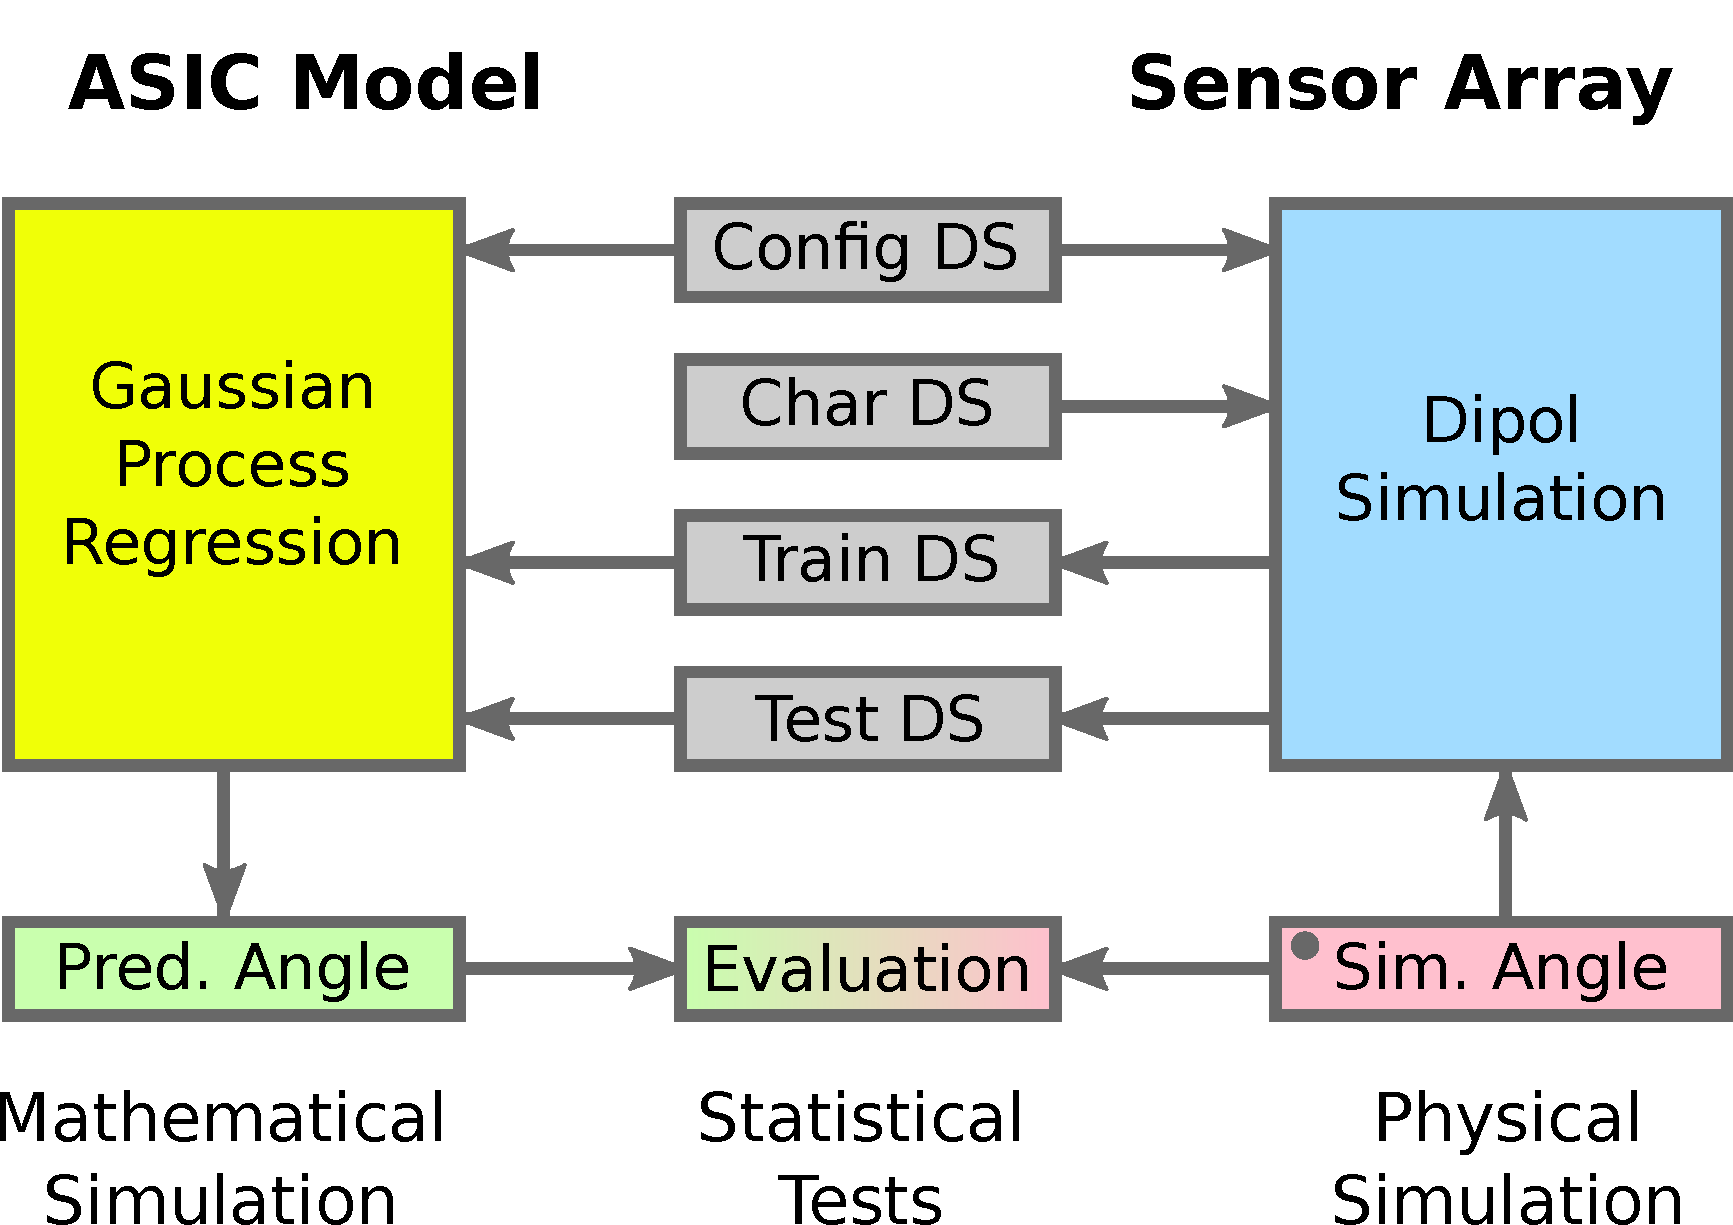
\includegraphics[width=0.7\linewidth]{chapters/images/3-SW-E-OExp/Software-Gesamtansicht}
	\caption[Simulationsaufbau im Überblick]{Simulationsaufbau im Überblick. Konzeptionelle Aufteilung der Simulationen für Sensor-Array und ASIC nach Simulationscharakter. Simulative Kopplung erfolgt, durch prozessierte Datensätze (DS). Eine statistische Auswertung bezieht sich auf angefahrene Simulationswinkel. Der Punkt kennzeichnet die Simulationswinkeleingabe und markiert den gedanklichen Startpunkt des Gesamtkonzepts.}
	\label{fig:software-gesamtansicht}
\end{figure}


Im ersten Simulationsschritt (Sensor-Array) werden Trainings- und Testdatensätze erzeugt. Die Datengenerierung in der Simulation basiert auf Charakterisierungsdatensätze. Diese stellen Technologieeigenschaften und Verhalten für die Simulation bereit, siehe \autoref{ch:tdk-datensatz}. Zur Datengenerierung sind physikalische Gleichungen aus \autoref{sec:sensor-array-simulation-dipol-feldgleichung} genutzt. Als zweiter Simulationsschritt (ASIC-Modell) folgt die Analyse der generierten Daten aus Schritt eins. Zur Analyse wird ein mathematisches Regressionsverfahren verwendet, siehe \autoref{sec:gauss-prozesse-regressionsverfahren}. Das Regressionsverfahren gewichtet Daten und macht entsprechende Vorhersagen gemäß eingestellter Regressionsziele und gewichteten Referenzdaten \autoref{ch:gpr-imp}. Das sind rein mathematische Vorhersagen für vorgegebene Funktionen. Ein physikalischer Gesamtbezug ist durch eine verbundene Auswertung beider Simulationsabschnitte herzustellen. Die Simulationssteuerung ist über einen gemeinsamen Konfigurationsdatensatz umgesetzt, siehe \autoref{tab:sensor-array-sim-params} und \autoref{tab:gpr-sim-params}. Die jeweiligen Parametergruppen sind entsprechend ihrer Zugehörigkeit partiell in den Simulationsbetrieb eingebunden. Der Konfigurationsdatensatz kann je nach Bedarf erzeugt und manipuliert werden. Zur Konfigurationsgenerierung ist das Skript aus \autoref{mcode:generateconfigmat} zu verwenden.


\clearpage


Die Zweischritt-Lösung bietet den Vorteil, dass zuerst verschiedenste Trainings- und Testdatensätze generiert werden können. Nachfolgende und voneinander variierende Simulationen basieren hierbei auf gleichen Datensätzen. Sie sind damit vergleichbar für weitere Auswertungen, Diagnosen oder Optimierungen. Ein empfohlener Arbeitsablauf ist in \autoref{mcode:simulation-workflow} festgehalten.
\newline
Zur Gestaltung der Simulations-Software ist ein modularer Ansatz nach \autoref{fig:blockschemasoftware} verfolgt worden. Das modulare Konzept erhöht die Wiederverwendbarkeit des Quellcodes. Es ermöglicht einzelne Quellcodebestandteile miteinander zu kombinieren. Die Einbindung und Ausführung der Quellcodemodule aus \autoref{mcode:source-code} erfolgt in Skripten des \autoref{mcode:executable-scripts}. Die Software ist als Projekt in der Multi-Paradigmen-Programmiersprache Matlab umgesetzt, siehe \autoref{ch:genutzte-sw}. Konzeptrichtlinien sind im \autoref{mcode:workflows} festgehalten. Zusätzliche Anweisungen zur Arbeitsweise, Projektpflege, Dokumentation und Vorlagen für Skripte und Funktionen sind beigefügt. Alle Entwicklungsschritte sind mittels Git-Versionsverwaltung kommentiert und nachvollziehbar dokumentiert. Jede Quellcode- und Skript-Datei ist nach festgelegten Konventionen geschrieben worden \cite{Johnson2014}. Es ermöglicht eine automatisierte Dokumentation des gesamten Software-Projekts in \autoref{ch:sw-doku}. Erzeugt ist diese mit Skripten aus \autoref{mcode:publishprojectfilestohtml} und \autoref{mcode:exportpublishedtopdf}.


\vspace{3mm}
\begin{figure}[bph]
	\centering
	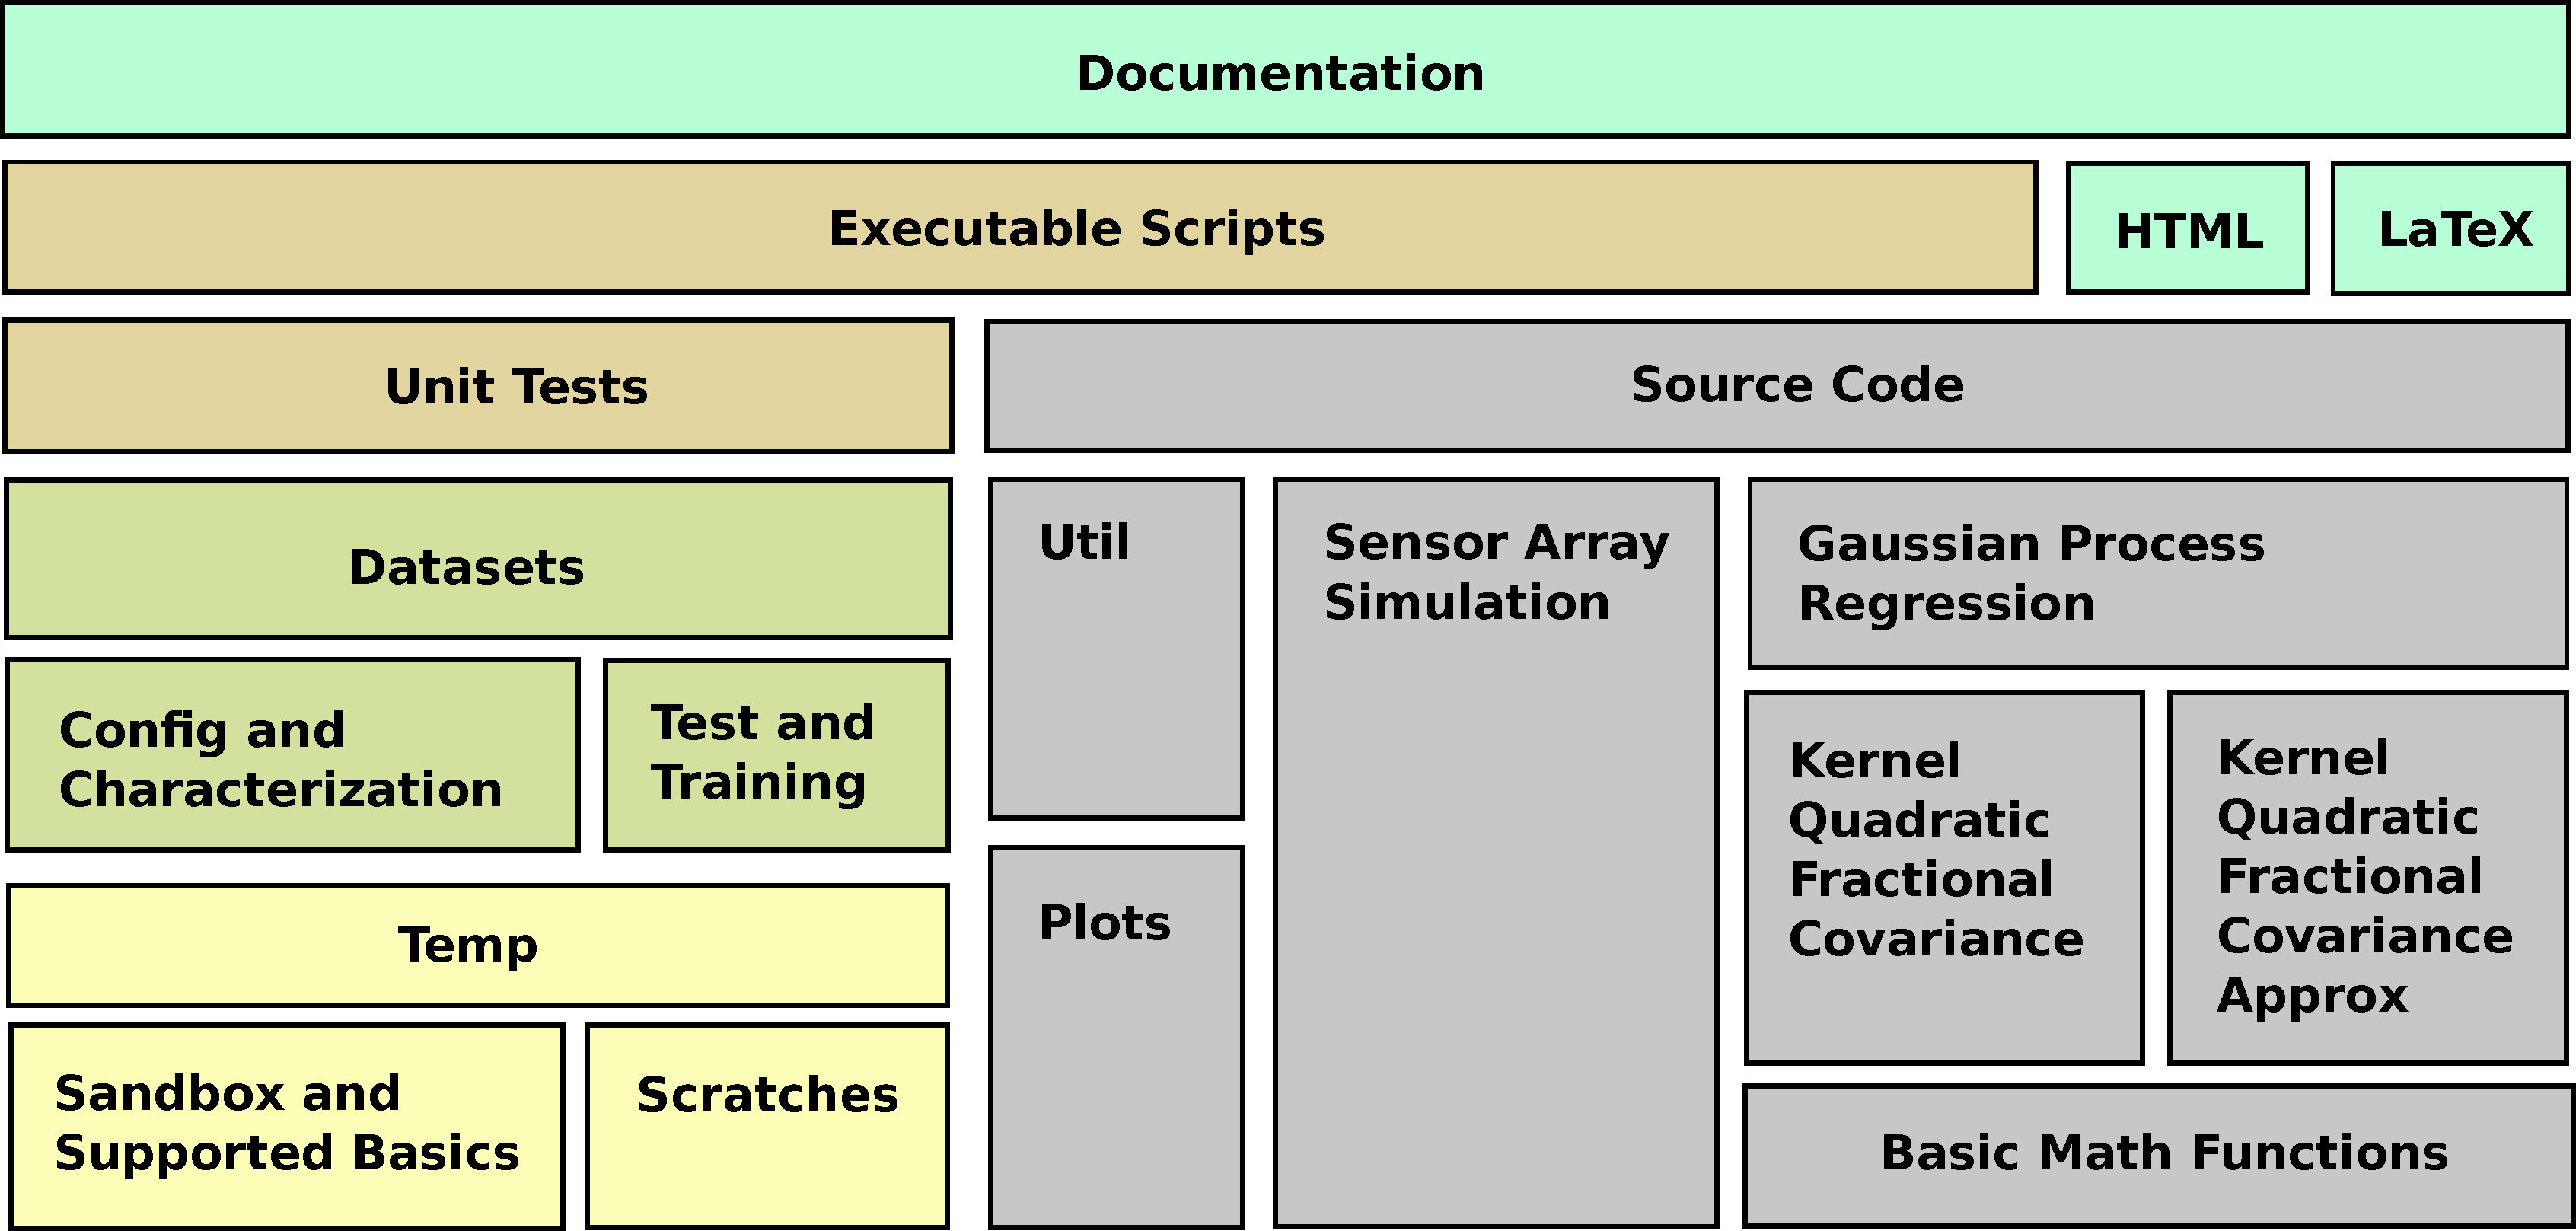
\includegraphics[width=\linewidth]{chapters/images/3-SW-E-OExp/Blockschema_Software}
	\caption[Blockschema Simulations-Software]{Blockschema Simulations-Software. Modulare Software-Gestaltung. Kernbestandteil ist funktionaler Quellcode. Quellcodemodule sind mit Datensätzen nach Bedarf in Skripten zu laden und ausführbar. Software-Dokumentation steht in HTML und LaTeX bereit. Als HTML ist diese in Matlab integriert. Entwurfsarbeiten sind nicht Bestandteil der Dokumentation, aber im Projektverzeichnis vorliegend.}
	\label{fig:blockschemasoftware}
\end{figure}


\clearpage

% !TEX root = ../thesis.tex
% simulation processes and execution
% @author Tobias Wulf
%

\section{Simulationsprozesse und Ausführung}\label{sec:sim-pro}


\subsection{Sensor-Array-Simulation}\label{sub:sensor-array-pro}


\begin{figure}[tbph]
	\centering
	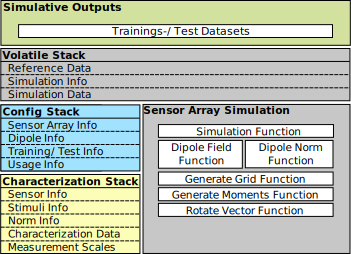
\includegraphics[width=0.7\linewidth]{chapters/images/3-SW-E-OExp/Blockschema_Sensor-Array}
	\caption[Blockschema Einbindung der Sensor-Array-Simulation]{Blockschema Einbindung der Sensor-Array-Simulation}
	\label{fig:blockschemasensor-array}
\end{figure}


\clearpage


\begin{figure}[tbph]
	\centering
	\includegraphics[width=\linewidth]{chapters/images/3-SW-E-OExp/Sensor-Array-Simulation}
	\caption[Sensor-Array-Simulation Prozessansicht]{Sensor-Array-Simulation Prozessansicht}
	\label{fig:sensor-array-simulation}
\end{figure}


\clearpage


\subsection{Gauß-Prozess-Regression}\label{sub:gpr-pro}


\paragraph{Trainingsphase}\label{par:gpr-training-pro}$~$\\


\begin{figure}[tbph]
	\centering
	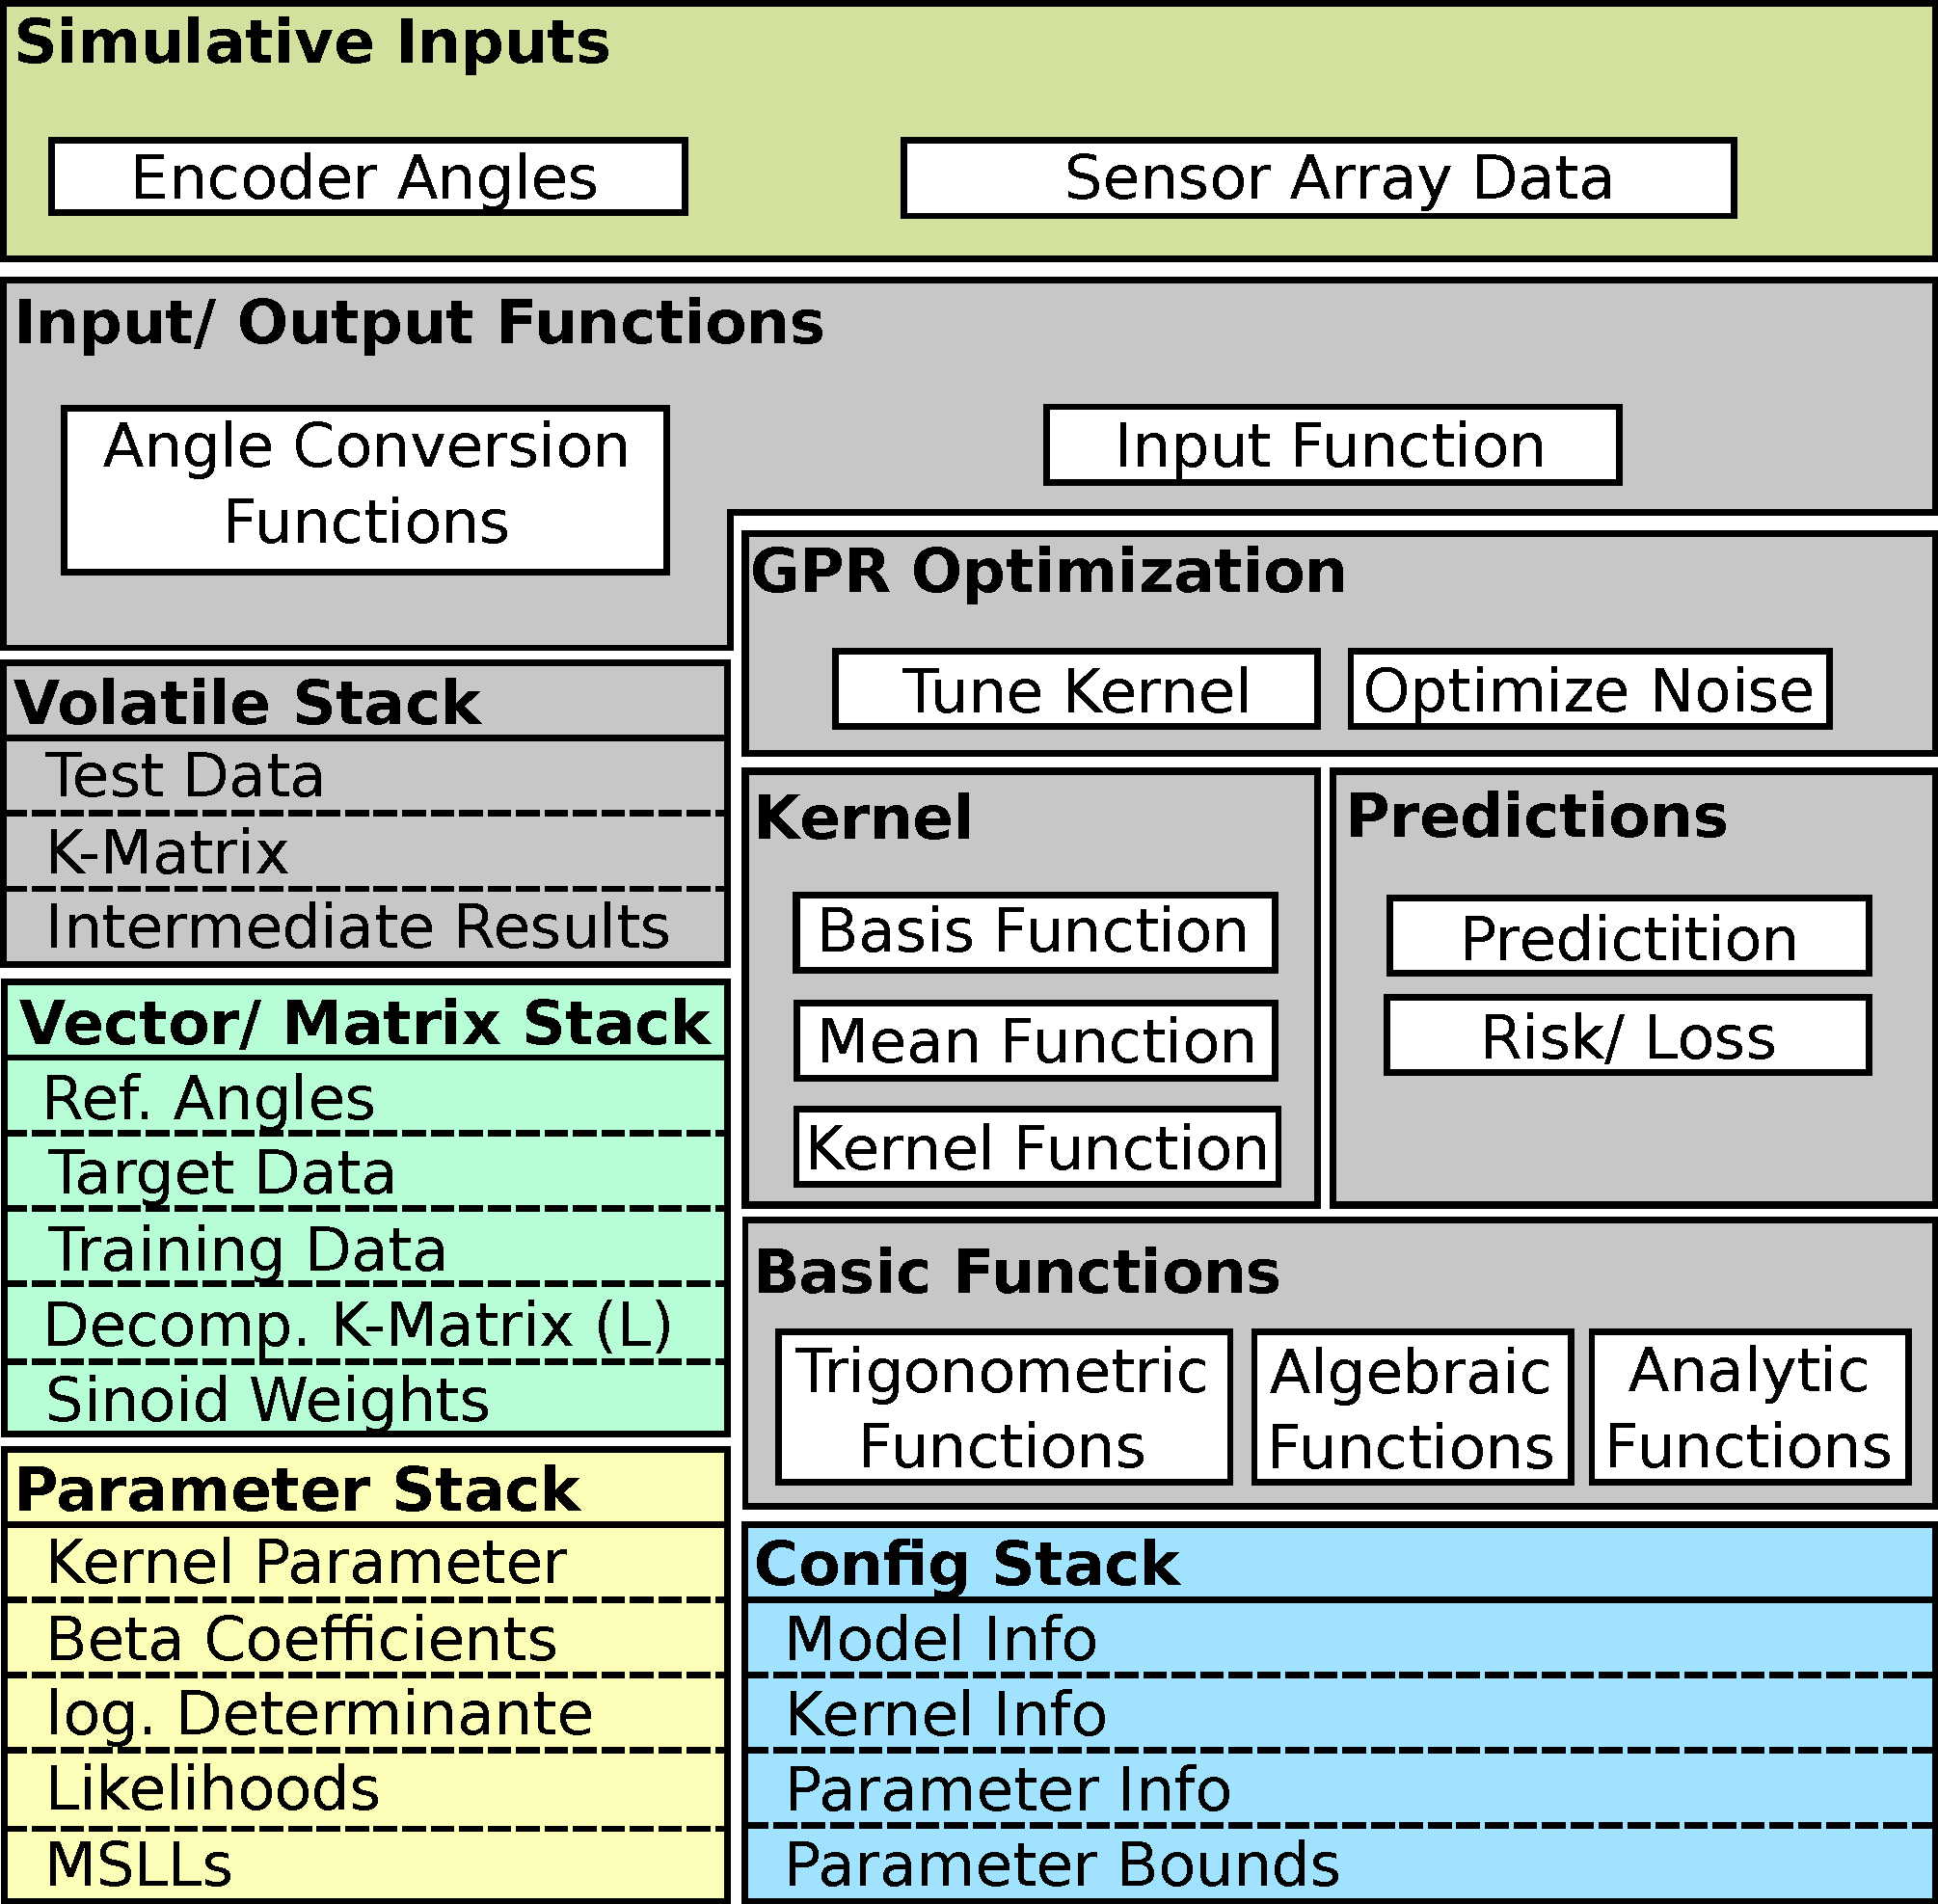
\includegraphics[width=0.7\linewidth]{chapters/images/3-SW-E-OExp/Blockschema_Trainingsphase}
	\caption[Blockschema Trainingsphase Regression]{Blockschema Trainingsphase Regression}
	\label{fig:blockschematrainingsphase}
\end{figure}


\clearpage


\begin{figure}[tbph]
	\centering
	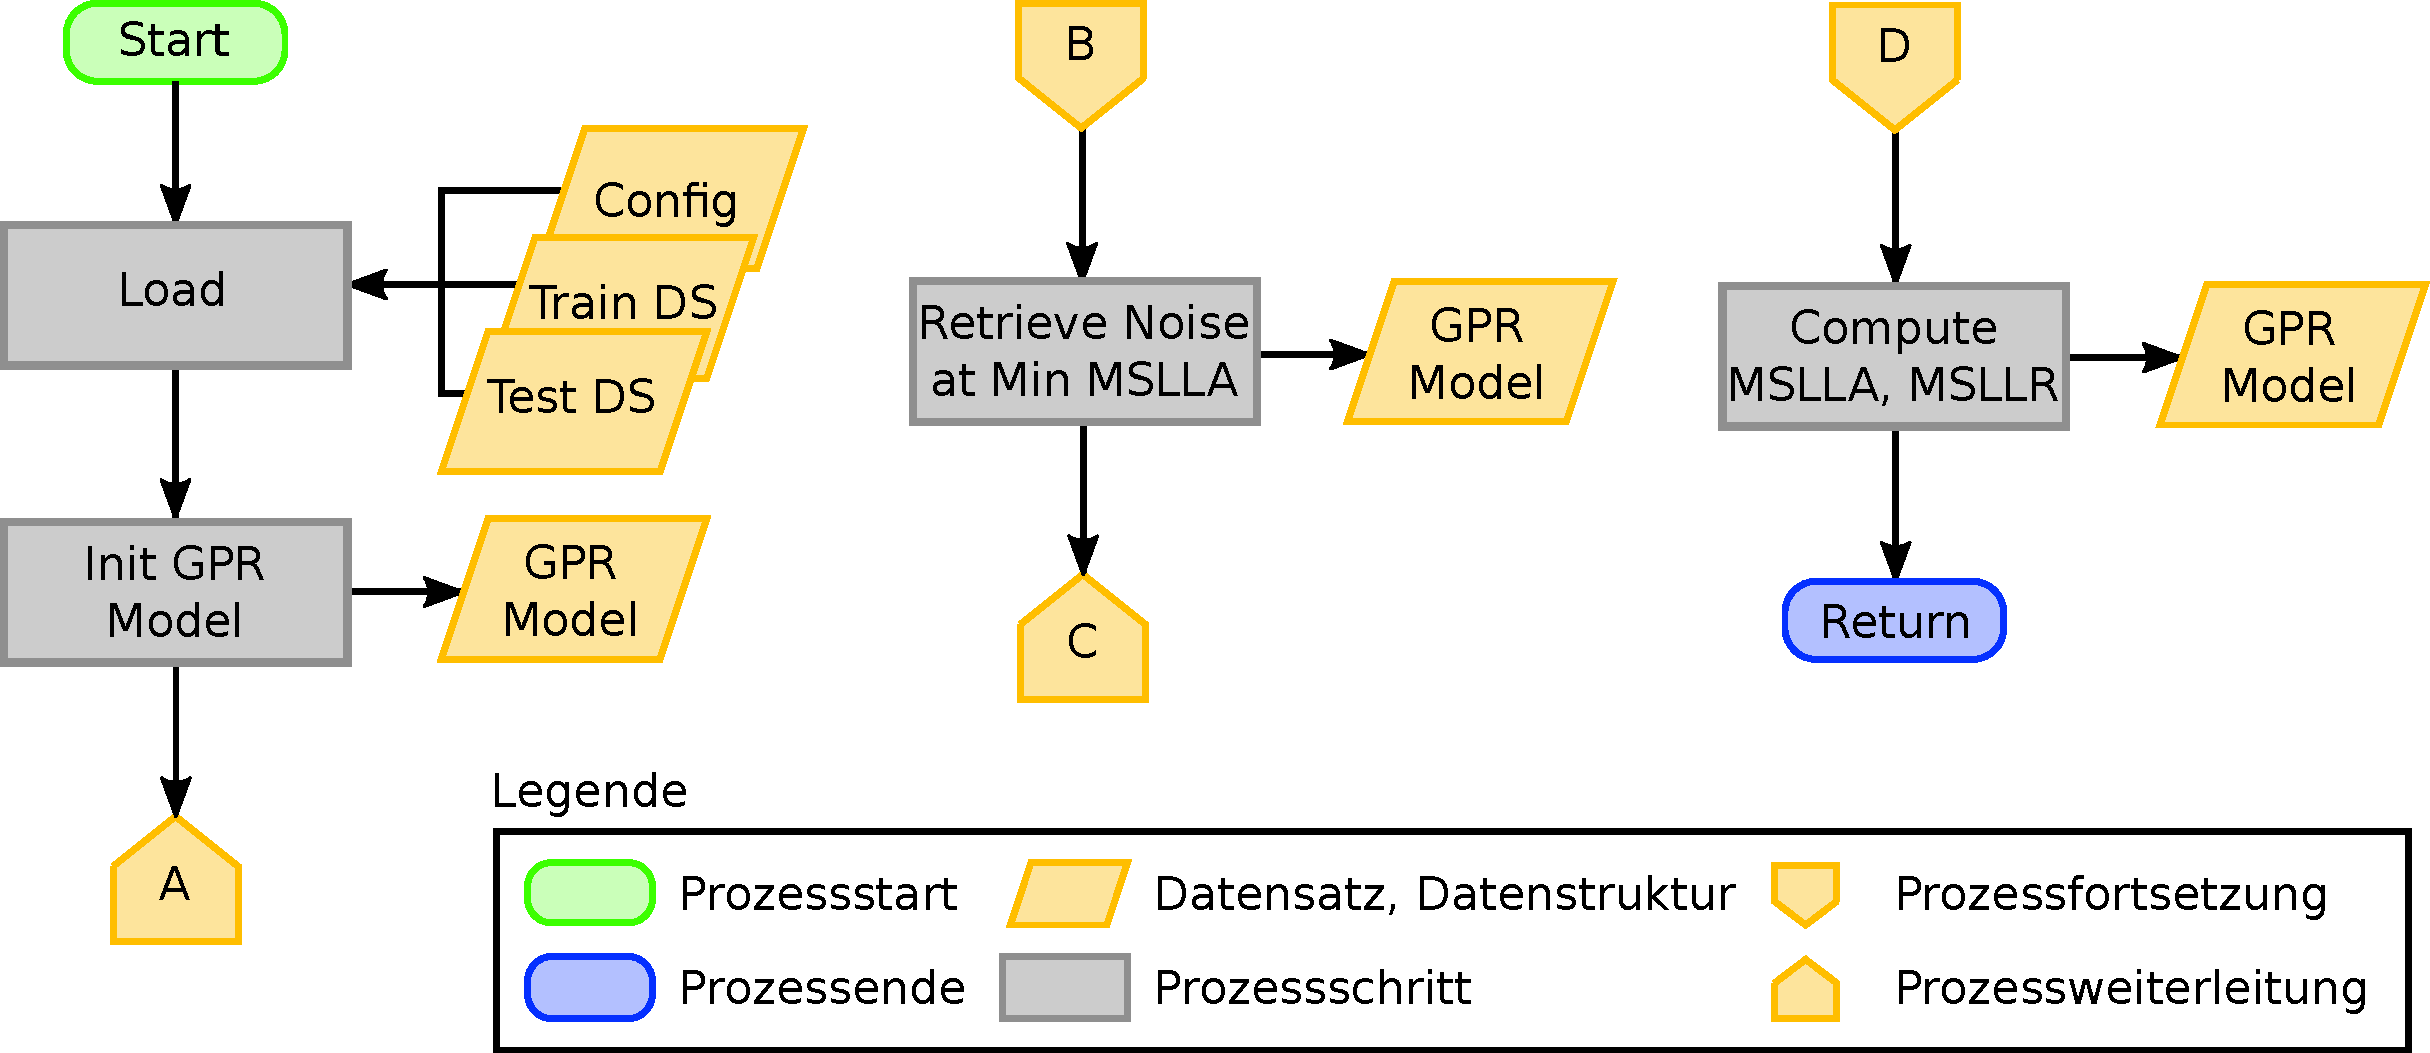
\includegraphics[width=.8\linewidth]{chapters/images/3-SW-E-OExp/GPR_Optimization}
	\caption[Regressionsoptimierung/ -Generalisierung Prozessansicht]{Regressionsoptimierung/ -Generalisierung Prozessansicht}
	\label{fig:gproptimization}
\end{figure}


\clearpage


\begin{figure}[htbp]
	\centering
	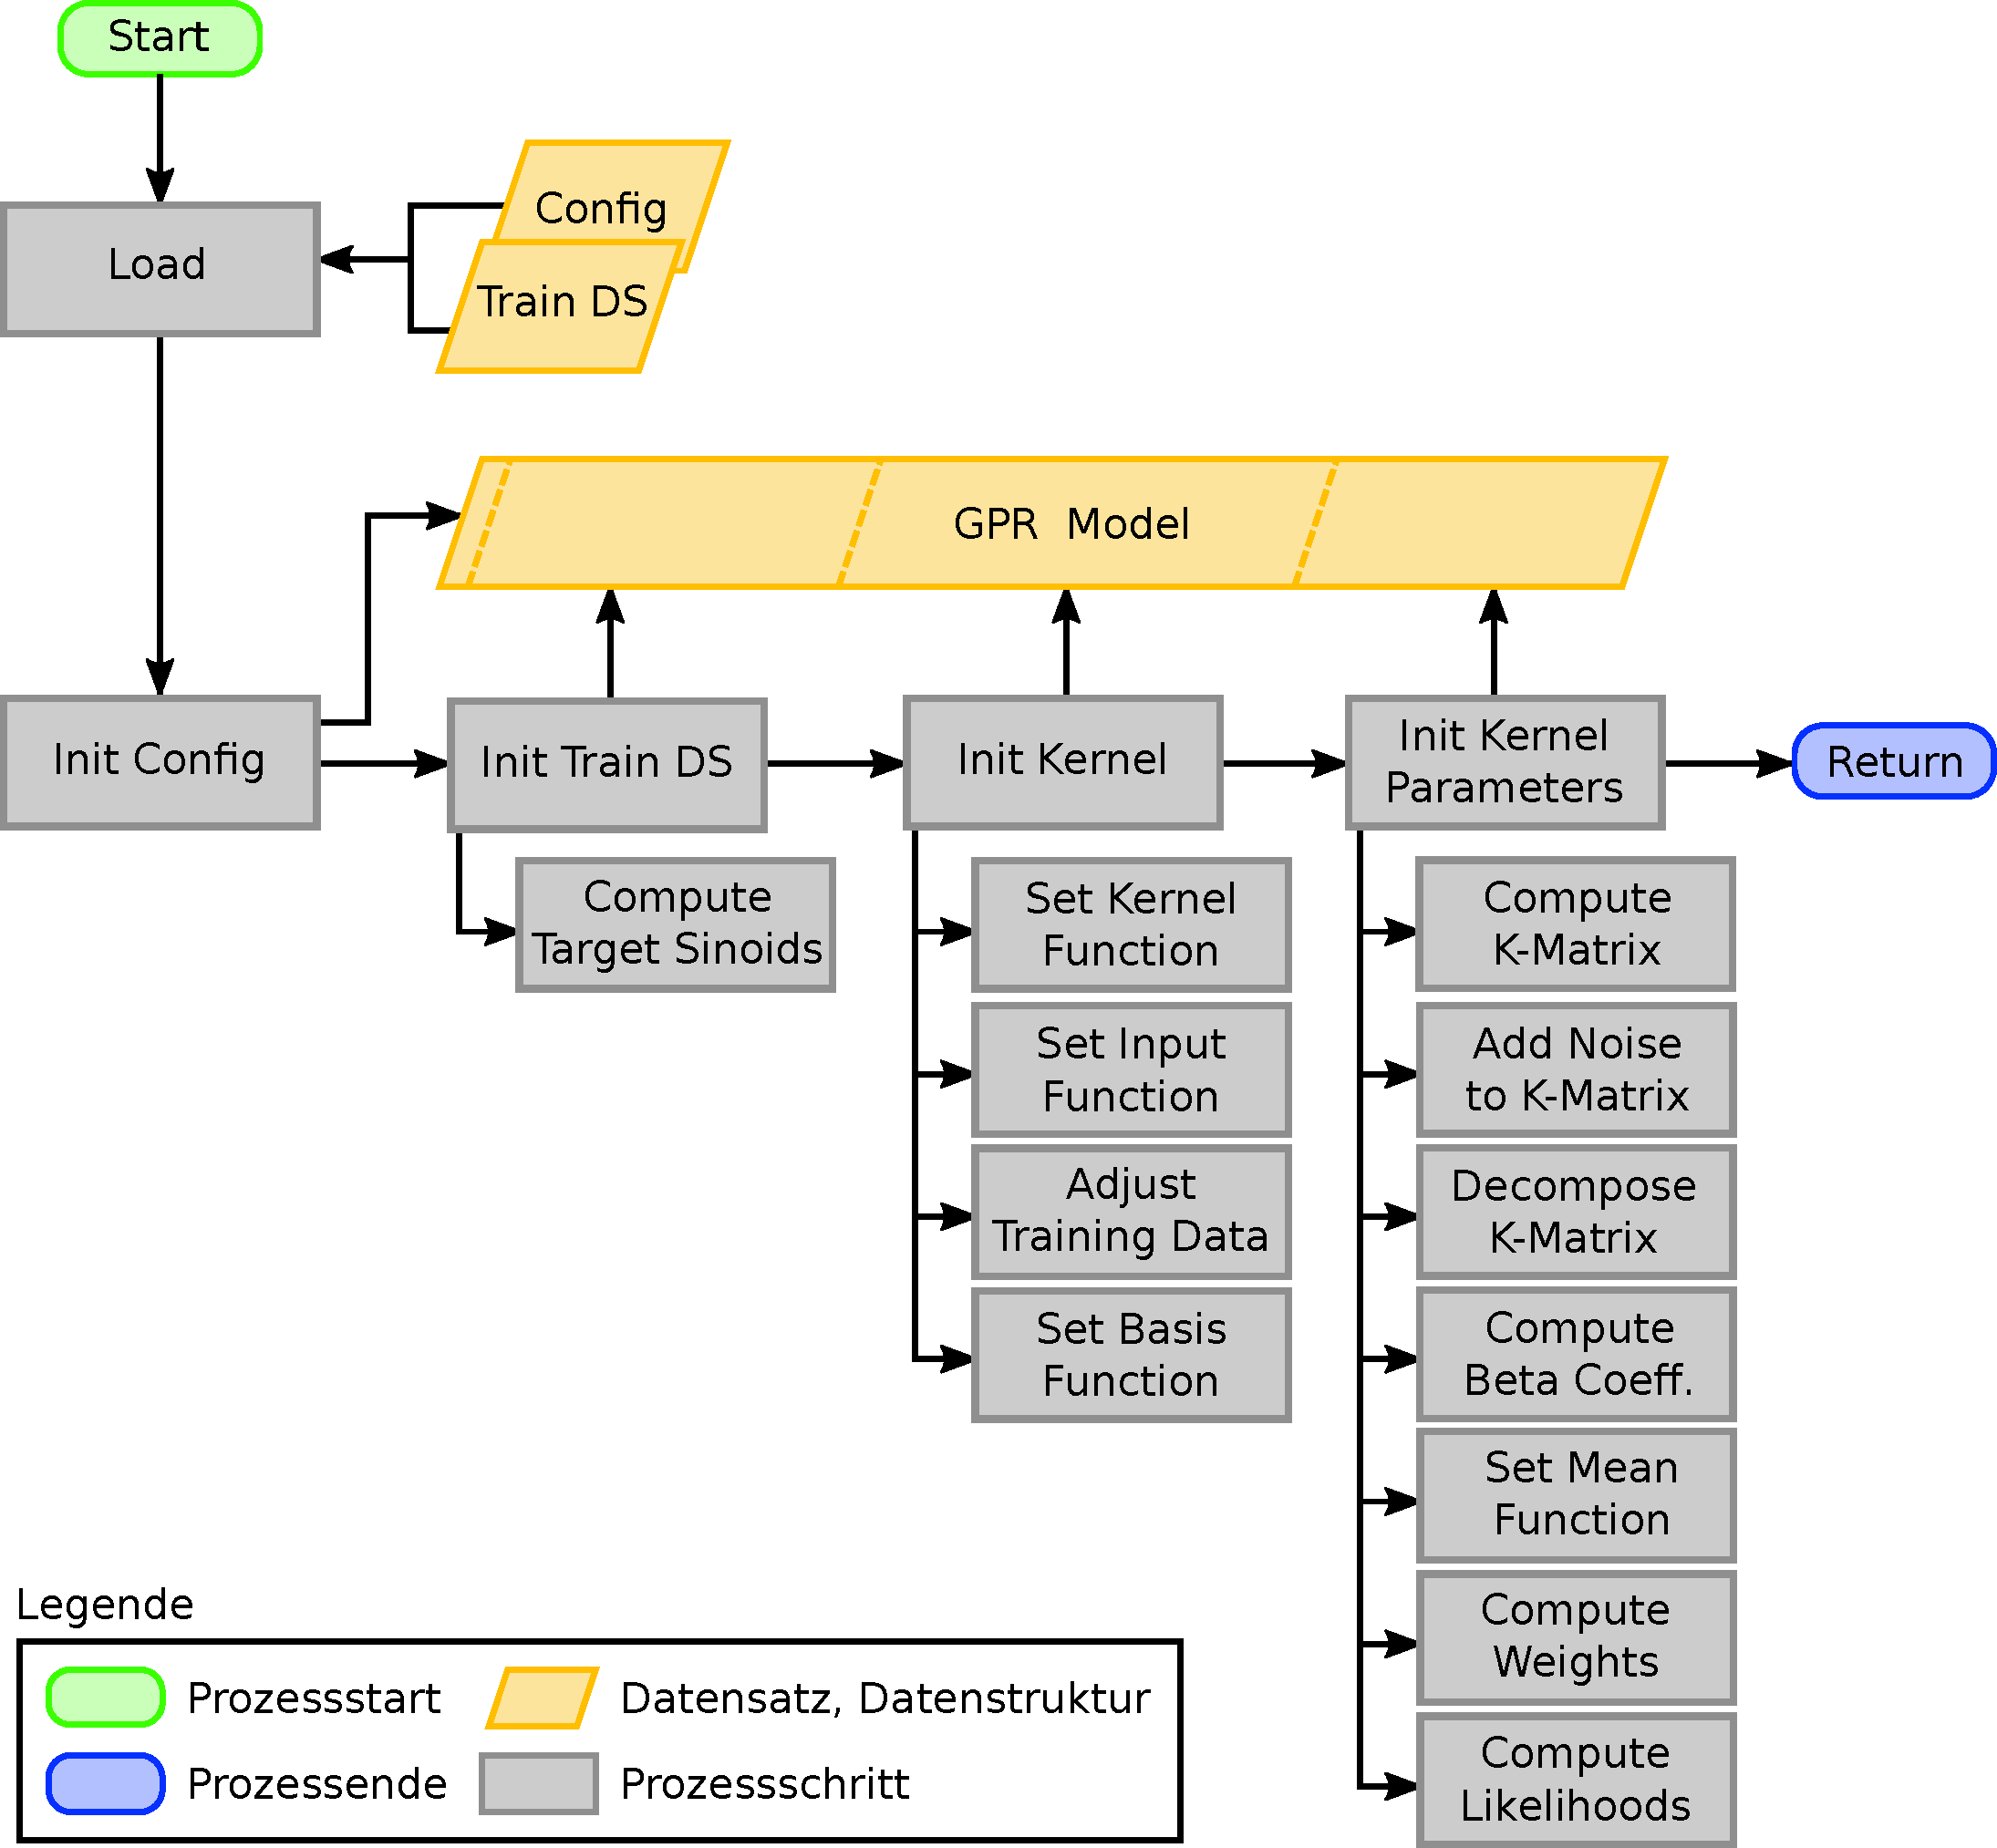
\includegraphics[width=0.7\linewidth]{chapters/images/3-SW-E-OExp/GPR_Initialization}
	\caption[Regressionsinitialisierung Prozessansicht]{Regressionsinitialisierung Prozessansicht}
	\label{fig:gprinitialization}
\end{figure}


\clearpage


\begin{figure}[tbph]
	\centering
	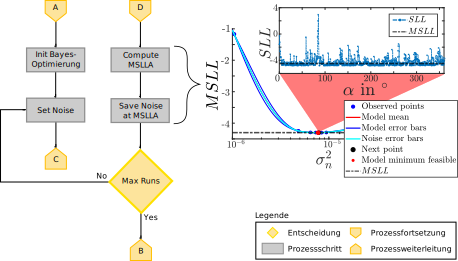
\includegraphics[width=0.85\linewidth]{chapters/images/3-SW-E-OExp/Noise_Optimization}
	\caption[Rauschniveauoptimierung Prozessansicht]{Rauschniveauoptimierung Prozessansicht}
	\label{fig:noiseoptimization}
\end{figure}


\clearpage


\begin{figure}[tbph]
	\centering
	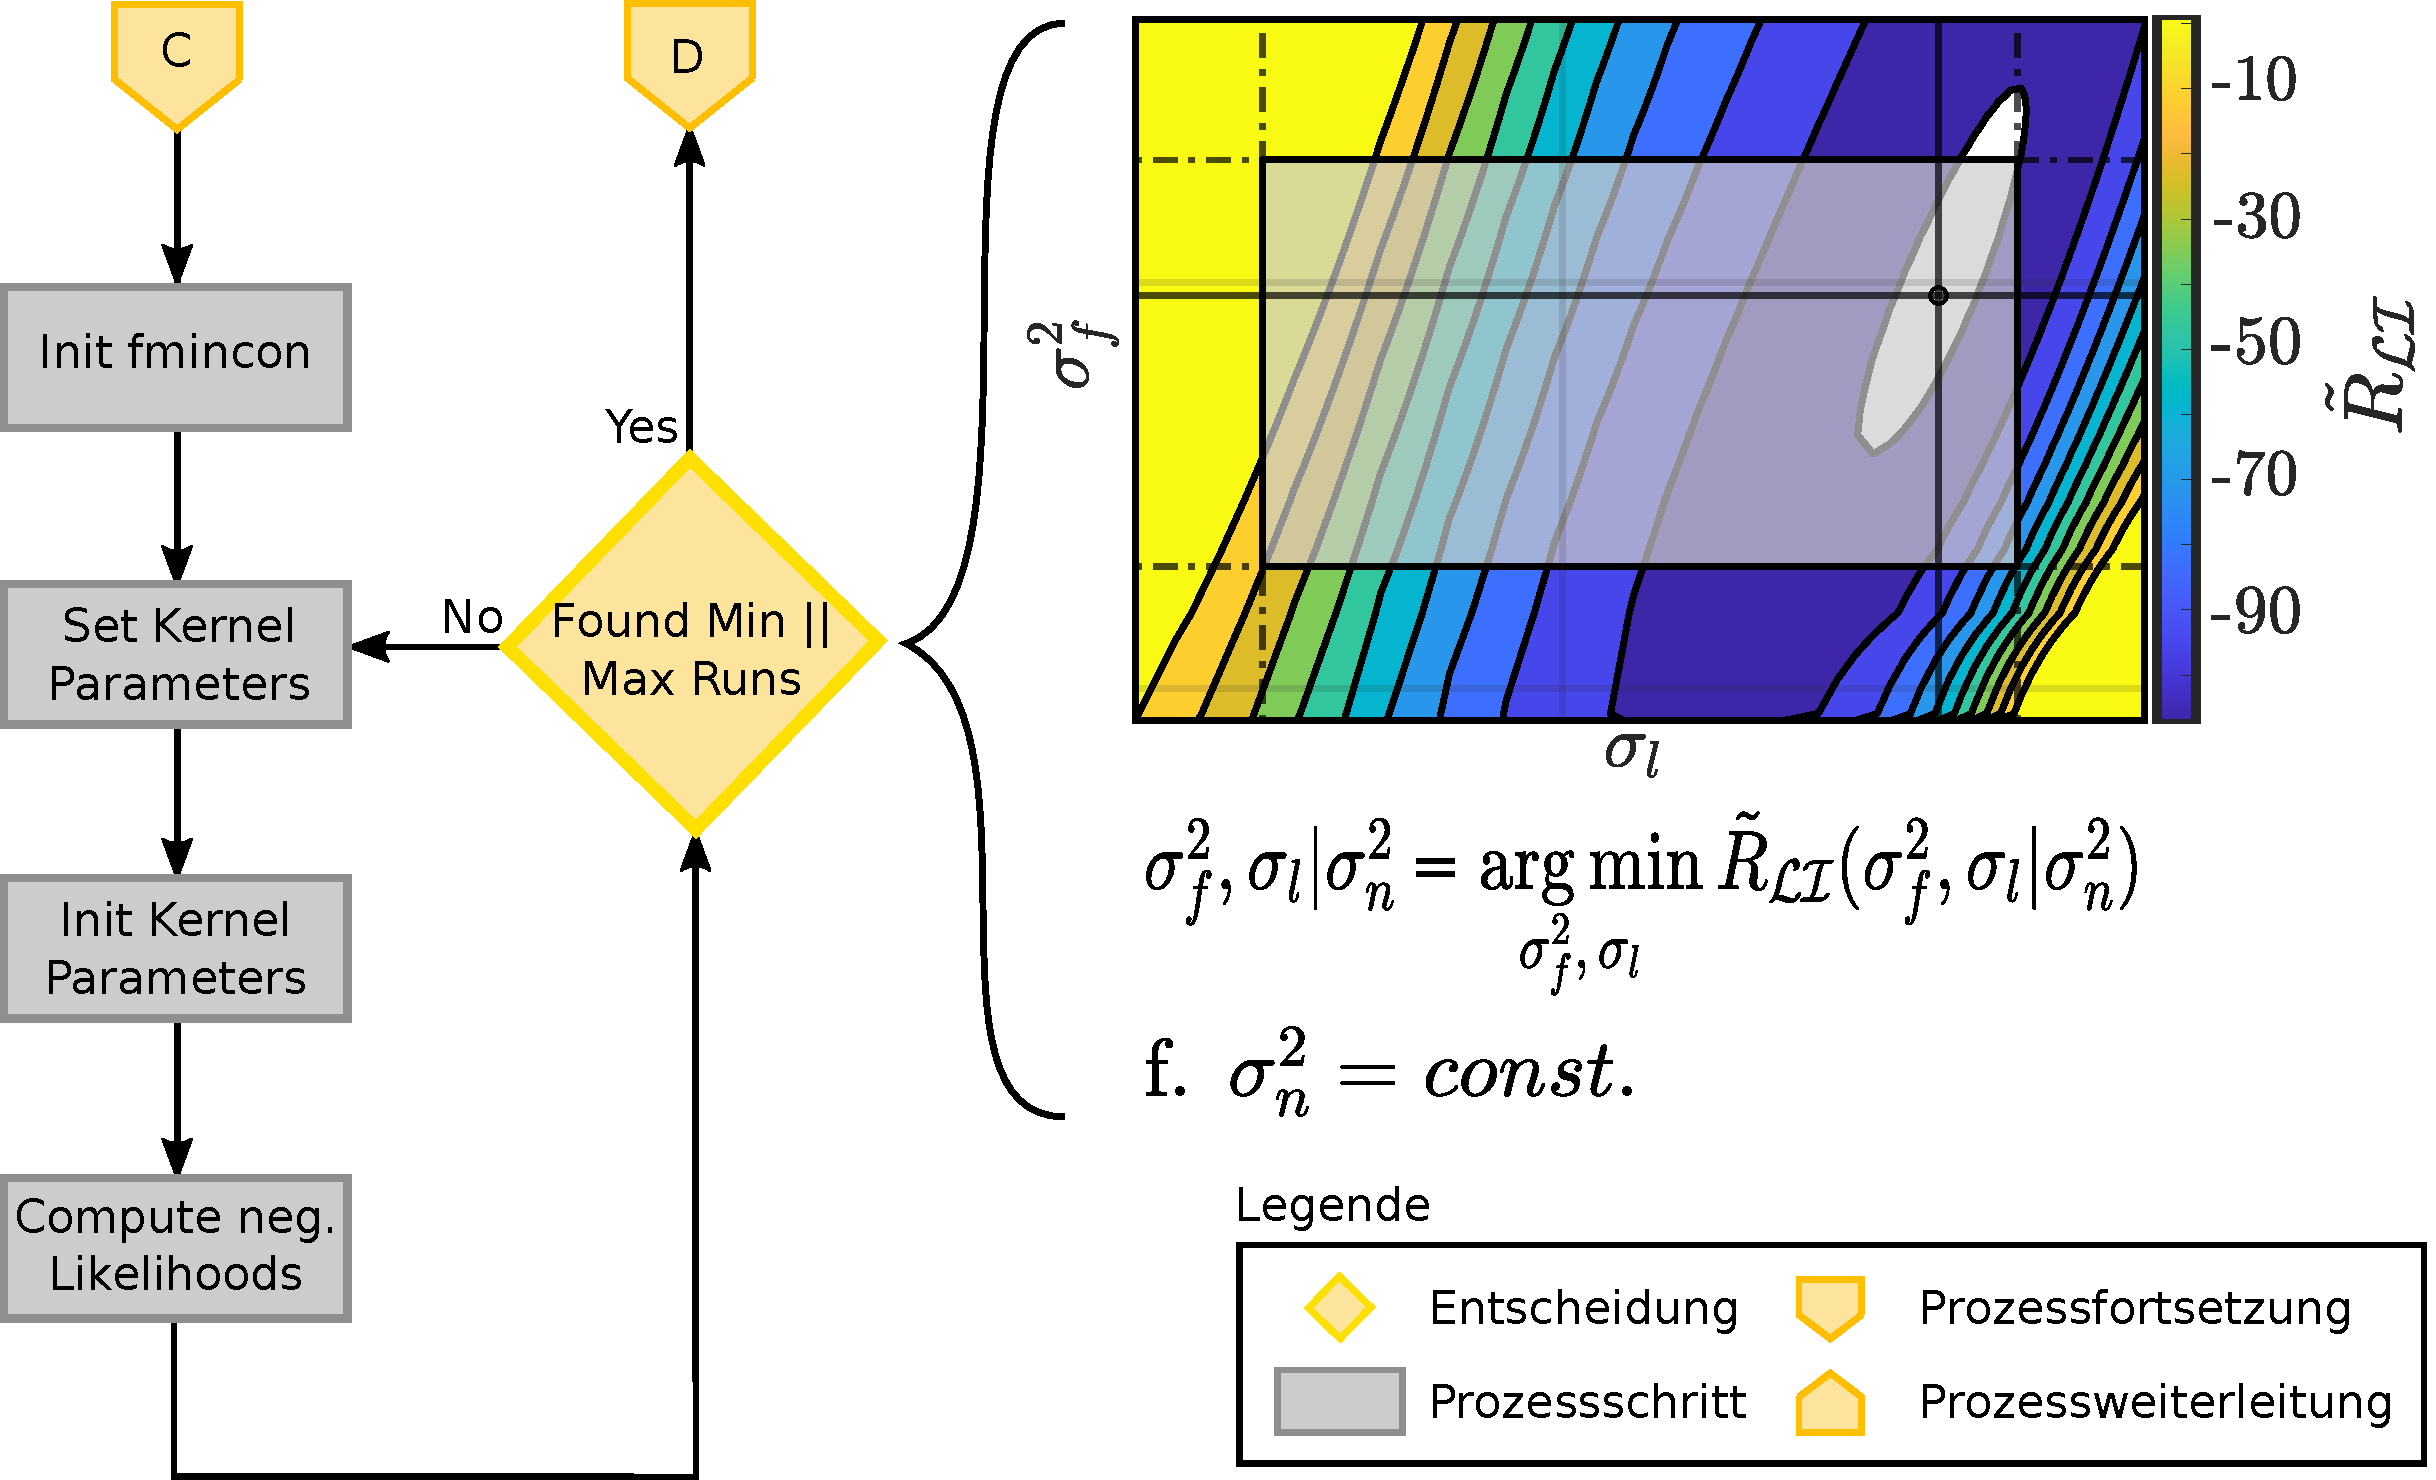
\includegraphics[width=0.8\linewidth]{chapters/images/3-SW-E-OExp/Kernel_Tuning}
	\caption[Regressionsparameteroptimierung Prozessansicht]{Regressionsparameteroptimierung Prozessansicht}
	\label{fig:kerneltuning}
\end{figure}


\clearpage


\paragraph{Arbeitsphase}\label{par:gpr-work-pro}$~$\\


\begin{figure}[tbph]
	\centering
	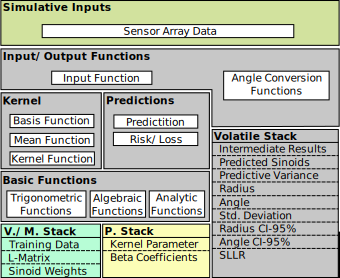
\includegraphics[width=0.7\linewidth]{chapters/images/3-SW-E-OExp/Blockschema_Workphase}
	\caption[Blockschema Arbeitsphase Regression]{Blockschema Arbeitsphase Regression}
	\label{fig:blockschemaworkphase}
\end{figure}


% !TEX root = ../thesis.tex
% testing and optimization experiments
% @author Tobias Wulf
%

\chapter{Erprobungs- und Optimierungsexperimente 0.0.2 26.04.2021}\label{ch:erprobungs-u-opt-exp}
	
	
\section{Vergleich der Kovarianzfunktionen}\label{sec:exp1}


\section{Anpassung der Referenzwinkelanzahl}\label{sec:exp2}


\section{Anpassung des Rauschniveaus}\label{sec:exp3}


\section{Anpassung der Parametergrenzen}\label{sec:exp4}


\section{Verhalten bei einfachen Fehllagen}\label{sec:exp5}
	
%	\begin{itemize}
%		\item Klassifizierung (Diagnose)
%		\item Stabilitätskriterium
%		\item Fehlererkennung Max. Mittelwert, Qualitätsmaß
%		\item Allg. Vorgehen "Batch-Job"
%		\item Konfigurierung der Simulationssoftware
%		\item Kategorisieren von Fehllagen, standardisierbar, mediale, maximale
%		\item Regressionsgrenzen durch Array-Technologie, Dämpfung Ellipsen
%	\end{itemize}
%
%\section{Festlegung des Startpunktes}\label{sec:festlegung-des-startpunktes}
%	\begin{itemize}
%		\item Startpunkt, 1. Position gleich Anlernpunkt für Trainingsphase
%		\item Auswahl des Senortyps
%		\item Konfigurierung des Magneten
%		\item Auswahl des GPR-Modells nach Optimierung
%		\item Konfigurierung des GPR-Modells mit ermittelten Parametern
%	\end{itemize}
%
%
%
%
%\section{Festlegung des Verfahrweges ohne Verkippung}\label{sec:festlegung-verfahrwe-ohne-verkippung}
%	\begin{itemize}
%		\item Vorbetrachtung des Magnetsfeldes 
%		\item Aufteilung in Sektoren
%		\item Abfahren in Z-Richtung ohne Versatz
%		\item Festlegen des X-Y-Versatzes, Symmetrie-Sektor		
%	\end{itemize}
%
%\section{Simulationsdurchführung}\label{sec:simulationsdurchfuehrung}
%	\begin{itemize}
%		\item Festhalten der Ergebnisse
%		\item Position, Winkelfehler (Max, Mittel), Qualitätsmaß (Max, Mittel)
%		\item Drift-Darstellung
%	\end{itemize}
	

% !TEX root = ../thesis.tex
% evaluation
% @author Tobias Wulf
%

\chapter{Auswertung}\label{ch:auswertung}

\section{Gegenüberstellung der GPR-Modelle}\label{sec:gegenueberstellung-gpr-modelle}
	\begin{itemize}
		\item Aufwand der Trainingsphase
		\item Nötige Parameter und zu Speichernde Werte
		\item Arbeitsphase, Genauigkeit, Fehlererkennung, Stabilität
	\end{itemize}
% !TEX root = ../thesis.tex
% summary and conclusion
% @author Tobias Wulf
%

\chapter{Zusammenfassung und Bewertung 0.0.1 13.01.2021}\label{ch:zusammenfassung}
\begin{itemize}
	\item Kurzdarstellung der Ergebnisse der Arbeit
	\item Offene Punkte und Probleme
	\item Ansätze zur Weiterführung für zukünftige Arbeiten
	\item Bewertung der Ergebnisse in Bezug auf die Anwendung
\end{itemize}


% List of figures here
\IListOfFigures

% List of tables here
\IListOfTables

% List glossary entries
\IGlossary

% List of accronyms here
\IListOfAccronyms

% List of symbols here
\IListOfSymbols

% List of used literature
\nocite{*}
\printbibliography
%\printbibliography[nottype=online, keyword={paper}, heading=subbibliography, title={Paper}]
%\printbibliography[nottype=online, keyword={thesis}, heading=subbibliography, title={Thesis}]
%\printbibliography[nottype=online, keyword={manual}, heading=subbibliography, title={Manual}]
%\printbibliography[type=online, keyword={webpage}, heading=subbibliography, title={Web-Recherche}]
% \bibliographystyle{plain}
%\bibliographystyle{dinat}
%\bibliography{literature/literature}

% Appendix
\appendix
\addcontentsline{toc}{part}{\appendixname}
\addtocontents{toc}{\protect\setcounter{tocdepth}{6}}
\setcounter{secnumdepth}{5}
% !TEX root = ../thesis.tex
% appendix TDK TAS2141-AAAB char dataset
% @author Tobias Wulf
%

\chapter{TDK TAS2141-AAAB Kennfelddatensatz 0.0.1 29.03.2021}\label{ch:tdk-datensatz}

Der Anhang beinhaltet die Kennfelddarstellung eines TAS2141-AAAB TMR-Winkelsensor der Firma TDK \cite{TDK2016}. Die 
Charakterisierung des Sensor-ICs ist mittels Kennfeldmethode \cite{Schuethe2019} vorgenommen worden. Das Ausmessen des 
TMR-Sensors hat im Labor der \gls{gl:ags} stattgefunden. Als Charakterisierungsergebnis liegt entsprechender Datensatz 
vor und dient in dieser Arbeit als Simulationsgrundlage für die Sensor-Array-Simulation. Der Datensatz ist von der 
\gls{gl:ags} zur Verfügung gestellt worden.


\vspace{5mm}
\begin{table}[!htbp]
	\centering
	%\resizebox{\textwidth}{!}{
	\begin{tabular}{l l l}
		\toprule
		\textbf{Eigenschaft}      & \textbf{Wert}    & \textbf{Einheit} \\
		\midrule
		$H_x$-Skala               & $-25 \ldots 25$  & $\SI{}{\kilo\ampere\per\metre}$ \\
		$H_y$-Skala               & $-25 \ldots 25$  & $\SI{}{\kilo\ampere\per\metre}$ \\
		\hline
		$H_x$-Schrittweite        & $0,1961$         & $\SI{}{\kilo\ampere\per\metre}$ \\
		$H_y$-Schrittweite        & $0,1961$         & $\SI{}{\kilo\ampere\per\metre}$ \\
		\hline
		Auflösung                 & $256 \times 256$ & Pixel \\
		Wertebereich $V(H_x,H_y)$ & Normiert         & $\SI{}{\milli\volt\per\volt}$ \\
		\hline
		Normfaktor                & $1\cdot 10^{-3}$ & $\SI{}{\per\milli\volt}$ \\
		Gain                      & 1                & - \\
		\hline
		Brückenverdrehung         & 90               & $\SI{}{\degree}$ \\
		Periodizität              & 360              & $\SI{}{\degree}$ \\
		\bottomrule		
	\end{tabular}%}
	\caption[Eckdaten TDK TAS2141-AAAB Kennfelder]{Eckdaten TDK TAS2141-AAAB Kennfelder}
\label{tab:tdk-char-data}
\end{table}


Die Charakterisierung mittels Kennfeldmethode generiert zwei Kennfeldpaare, zu sehen in \autoref{fig:tdkkennfelder}. 
Das erste Kennfeldpaar a) und c) referenziert sich aus dem steigenden Messverlauf, der amplitudenmodulierten 
$H_x$-/ $H_y$-Stimuli. Das zweite b) und d) setzt sich aus dem fallenden Stimuli zusammen. Ein Kennfeld repräsentiert 
dabei eine Wheatstone-Brücke des Winkelsensors \cite{Schuethe2019}. Bedingt durch die Verdrehung beider Brücken 
\cite{TDK2016}, ist ein entsprechendes Kennfeldpaar zueinander um $\SI{90}{\degree}$ verdreht.
Die Kennfelder besitzen, je ein Minimum und Maximum, dass bei Abfahren eines Kreises auf einem Kennfeld zur 
$\SI{360}{\degree}$ Periodizität führt. Die Kennfelder entsprechen somit dem Kernverhalten des Winkelsensors 
\cite{TDK2016}. \autoref{tab:tdk-char-data} fasst die Grundeigenschaften der Kennfelder zusammen. Beim zusammensetzen 
der Kennfelder, sind die gemessen Ausgangsspannungen normiert und von Offsets bereinigt worden. Das erleichtert den 
Simulationseinsatz mit variablen Betriebsspannungen. So können für beliebige Feldstärken, Ausgangsspannungen nach 
\autoref{eq:vout-tdk} aus den Kennfeldern entnommen werden.


\begin{equation}\label{eq:vout-tdk}
	\mathbf{V_{cos,sin}(H_x,H_y) = Gain \cdot Normfaktor \cdot V(H_x,H_y) \cdot V_{CC} + V_{Offset}}
\end{equation}


\begin{figure}[bph]
	\centering
	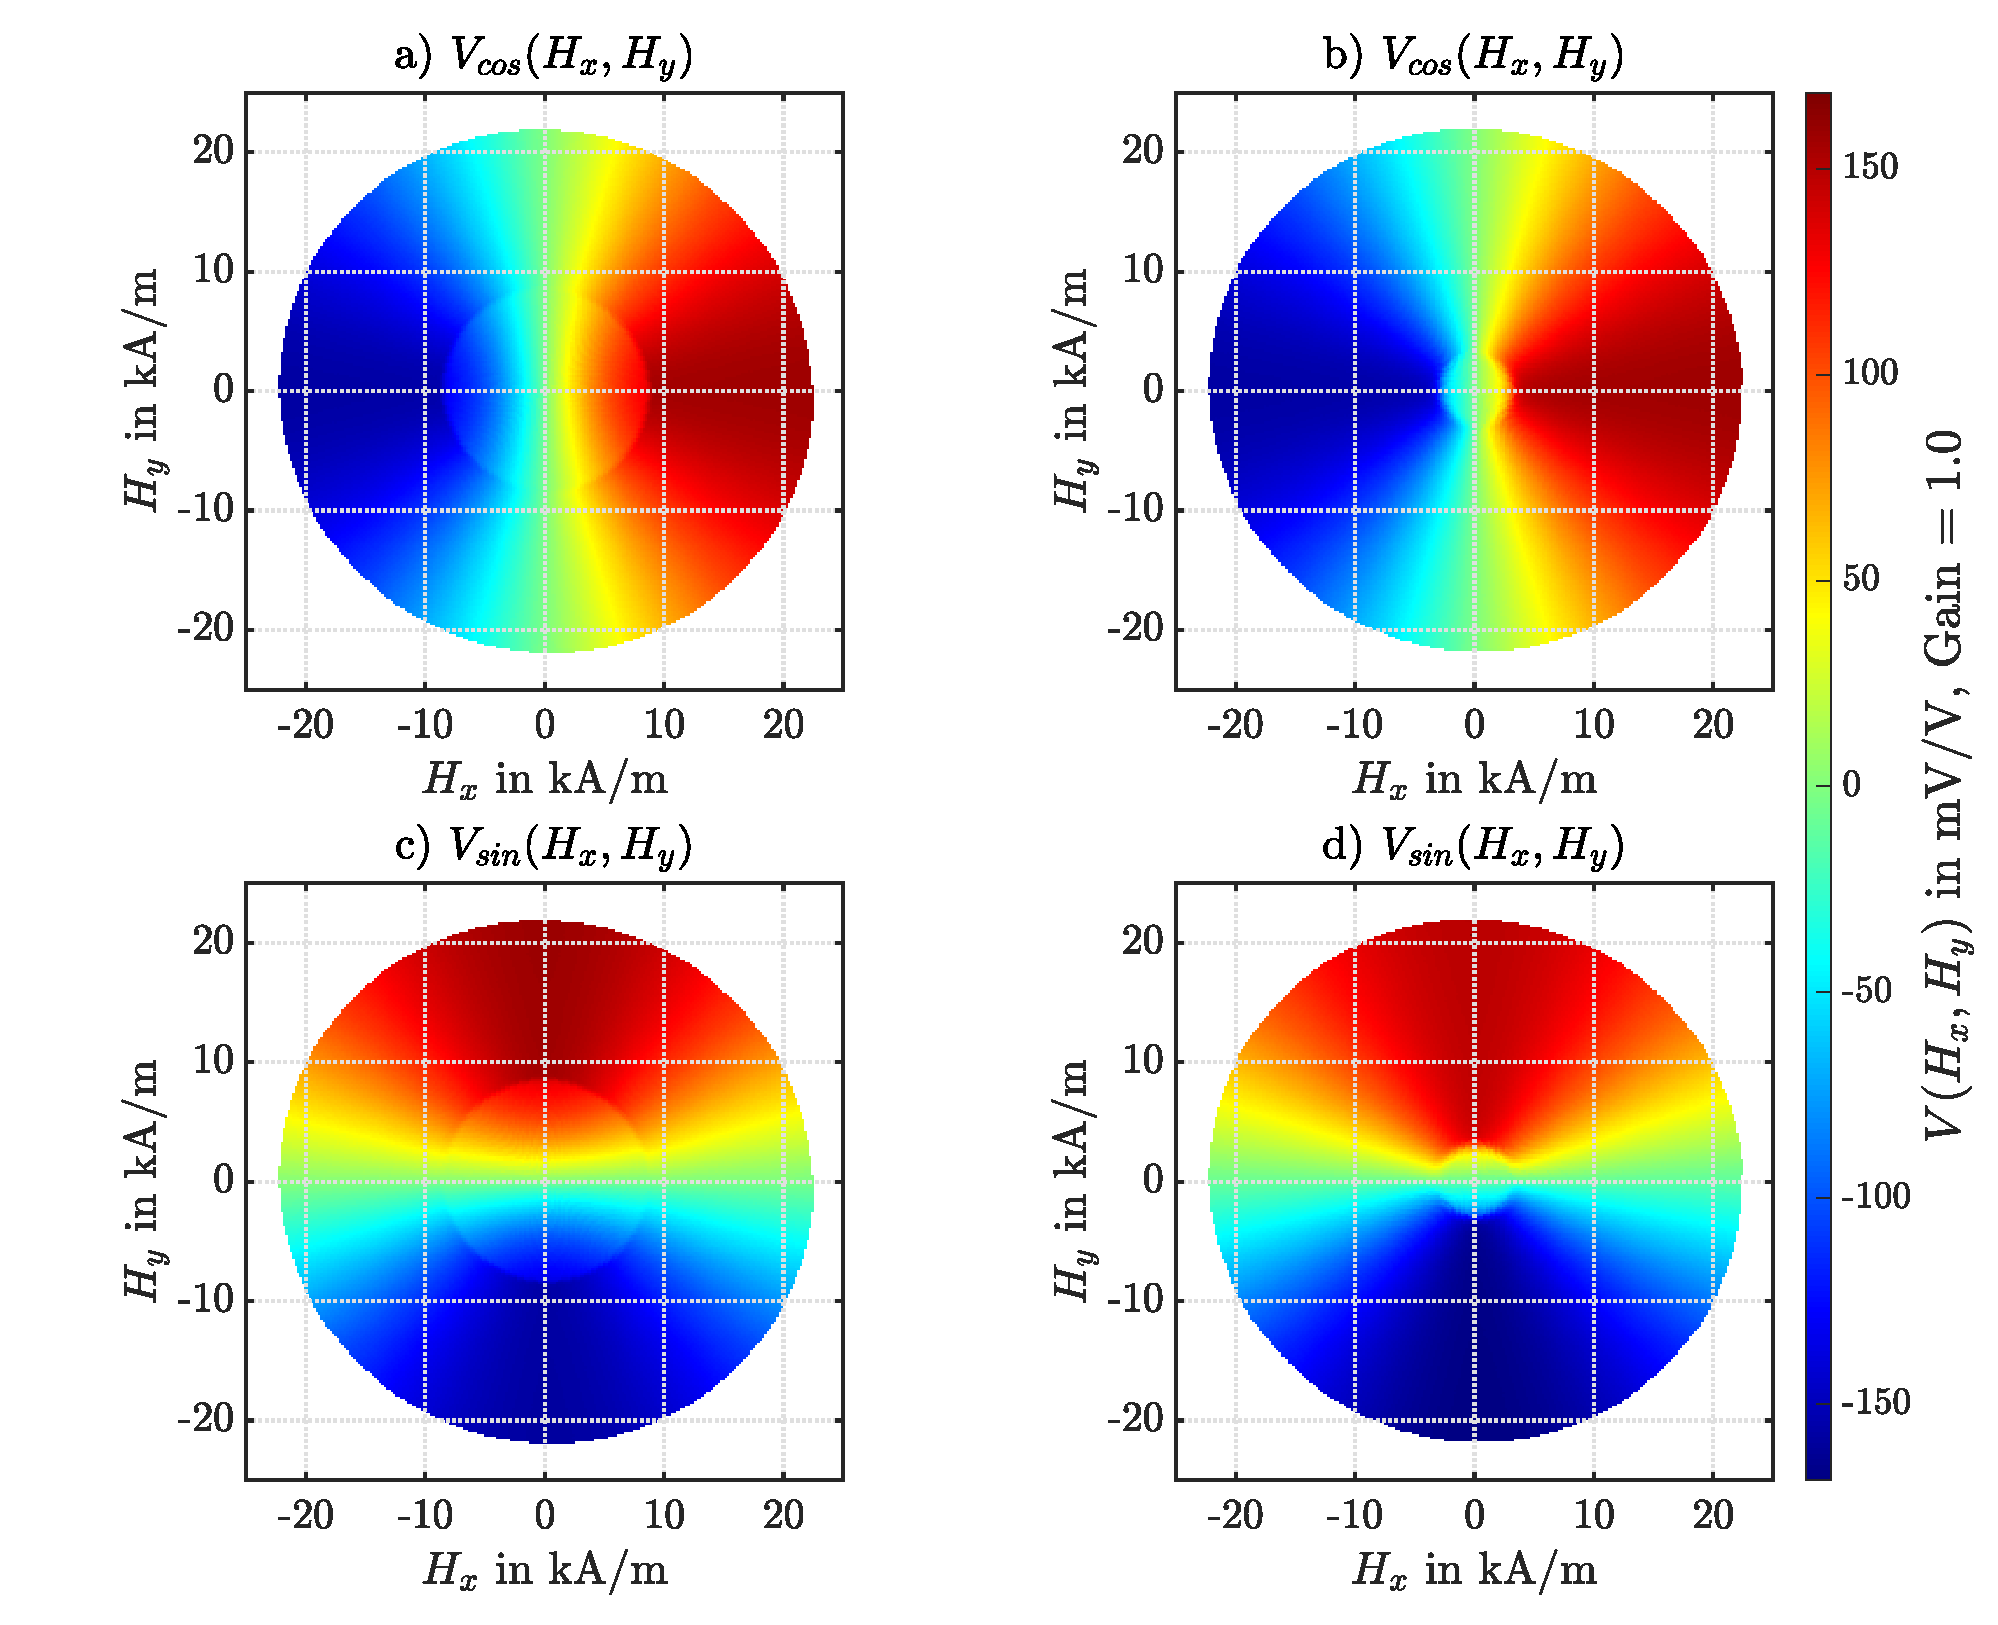
\includegraphics[width=.95\linewidth]{appendix/images/3-TDK/TDK_Kennfelder}
	\caption[TDK TAS2141-AAAB Brückenkennfelder]{TDK TAS2141-AAAB Brückenkennfelder. Kennfelder der Cosinus-Brücke a) 
		und b). Kennfelder der Sinus-Brücke c) und d). a) und c) gewonnen aus steigenden Amplitudenmodulation. b) und 
		d) gewonnen fallenden Modulation. Die Kennfelder sind normiert in $\SI{}{\milli\volt\per\volt}$. Grafik 
		nachempfunden 
		aus \cite{Schuethe2019}.}
	\label{fig:tdkkennfelder}
\end{figure}


\clearpage


Im Vergleich der Kennfeldpaare biete sich das erste aus aus \autoref{fig:tdkkennfelder} a) und c) für eine Simulation 
an. Die Kennfelder besitzen größere Plateauflächen \cite{Schuethe2019}. In \autoref{fig:tdkkennfeldsteigend} a) und c) 
ist das Kennfeldpaar nochmals gesondert dargestellt. Für das Kennfeld, der Cosinus-Wheatstone-Brücke in a), sind 
Querschnitte für variable $H_x$- und verschieden konstante $H_y$-Feldstärken in b) aufgetragen. Das gleiche vice versa 
in d) für Sinus-Wheatstone-Brücke aus c). Die Plateau-Grenzen liegen in $H_x$- und $H_y$-Richtung ca. bei 
$\pm\SI{8,5}{\kilo\ampere\per\metre}$ und sind als Limits in \autoref{fig:tdkkennfeldsteigend} b) und d) 
gekennzeichnet. Es zeigt sich ein annähernd linearer Bereich für die Übertragungskennlinien bei $H_{x,y} 
= \SI{0}{\kilo\ampere\per\metre}$. Dieser Arbeitsbereich ist für die Simulation einzustellen \cite{Schuethe2019}.


\vspace{5mm}
\begin{figure}[bph]
	\centering
	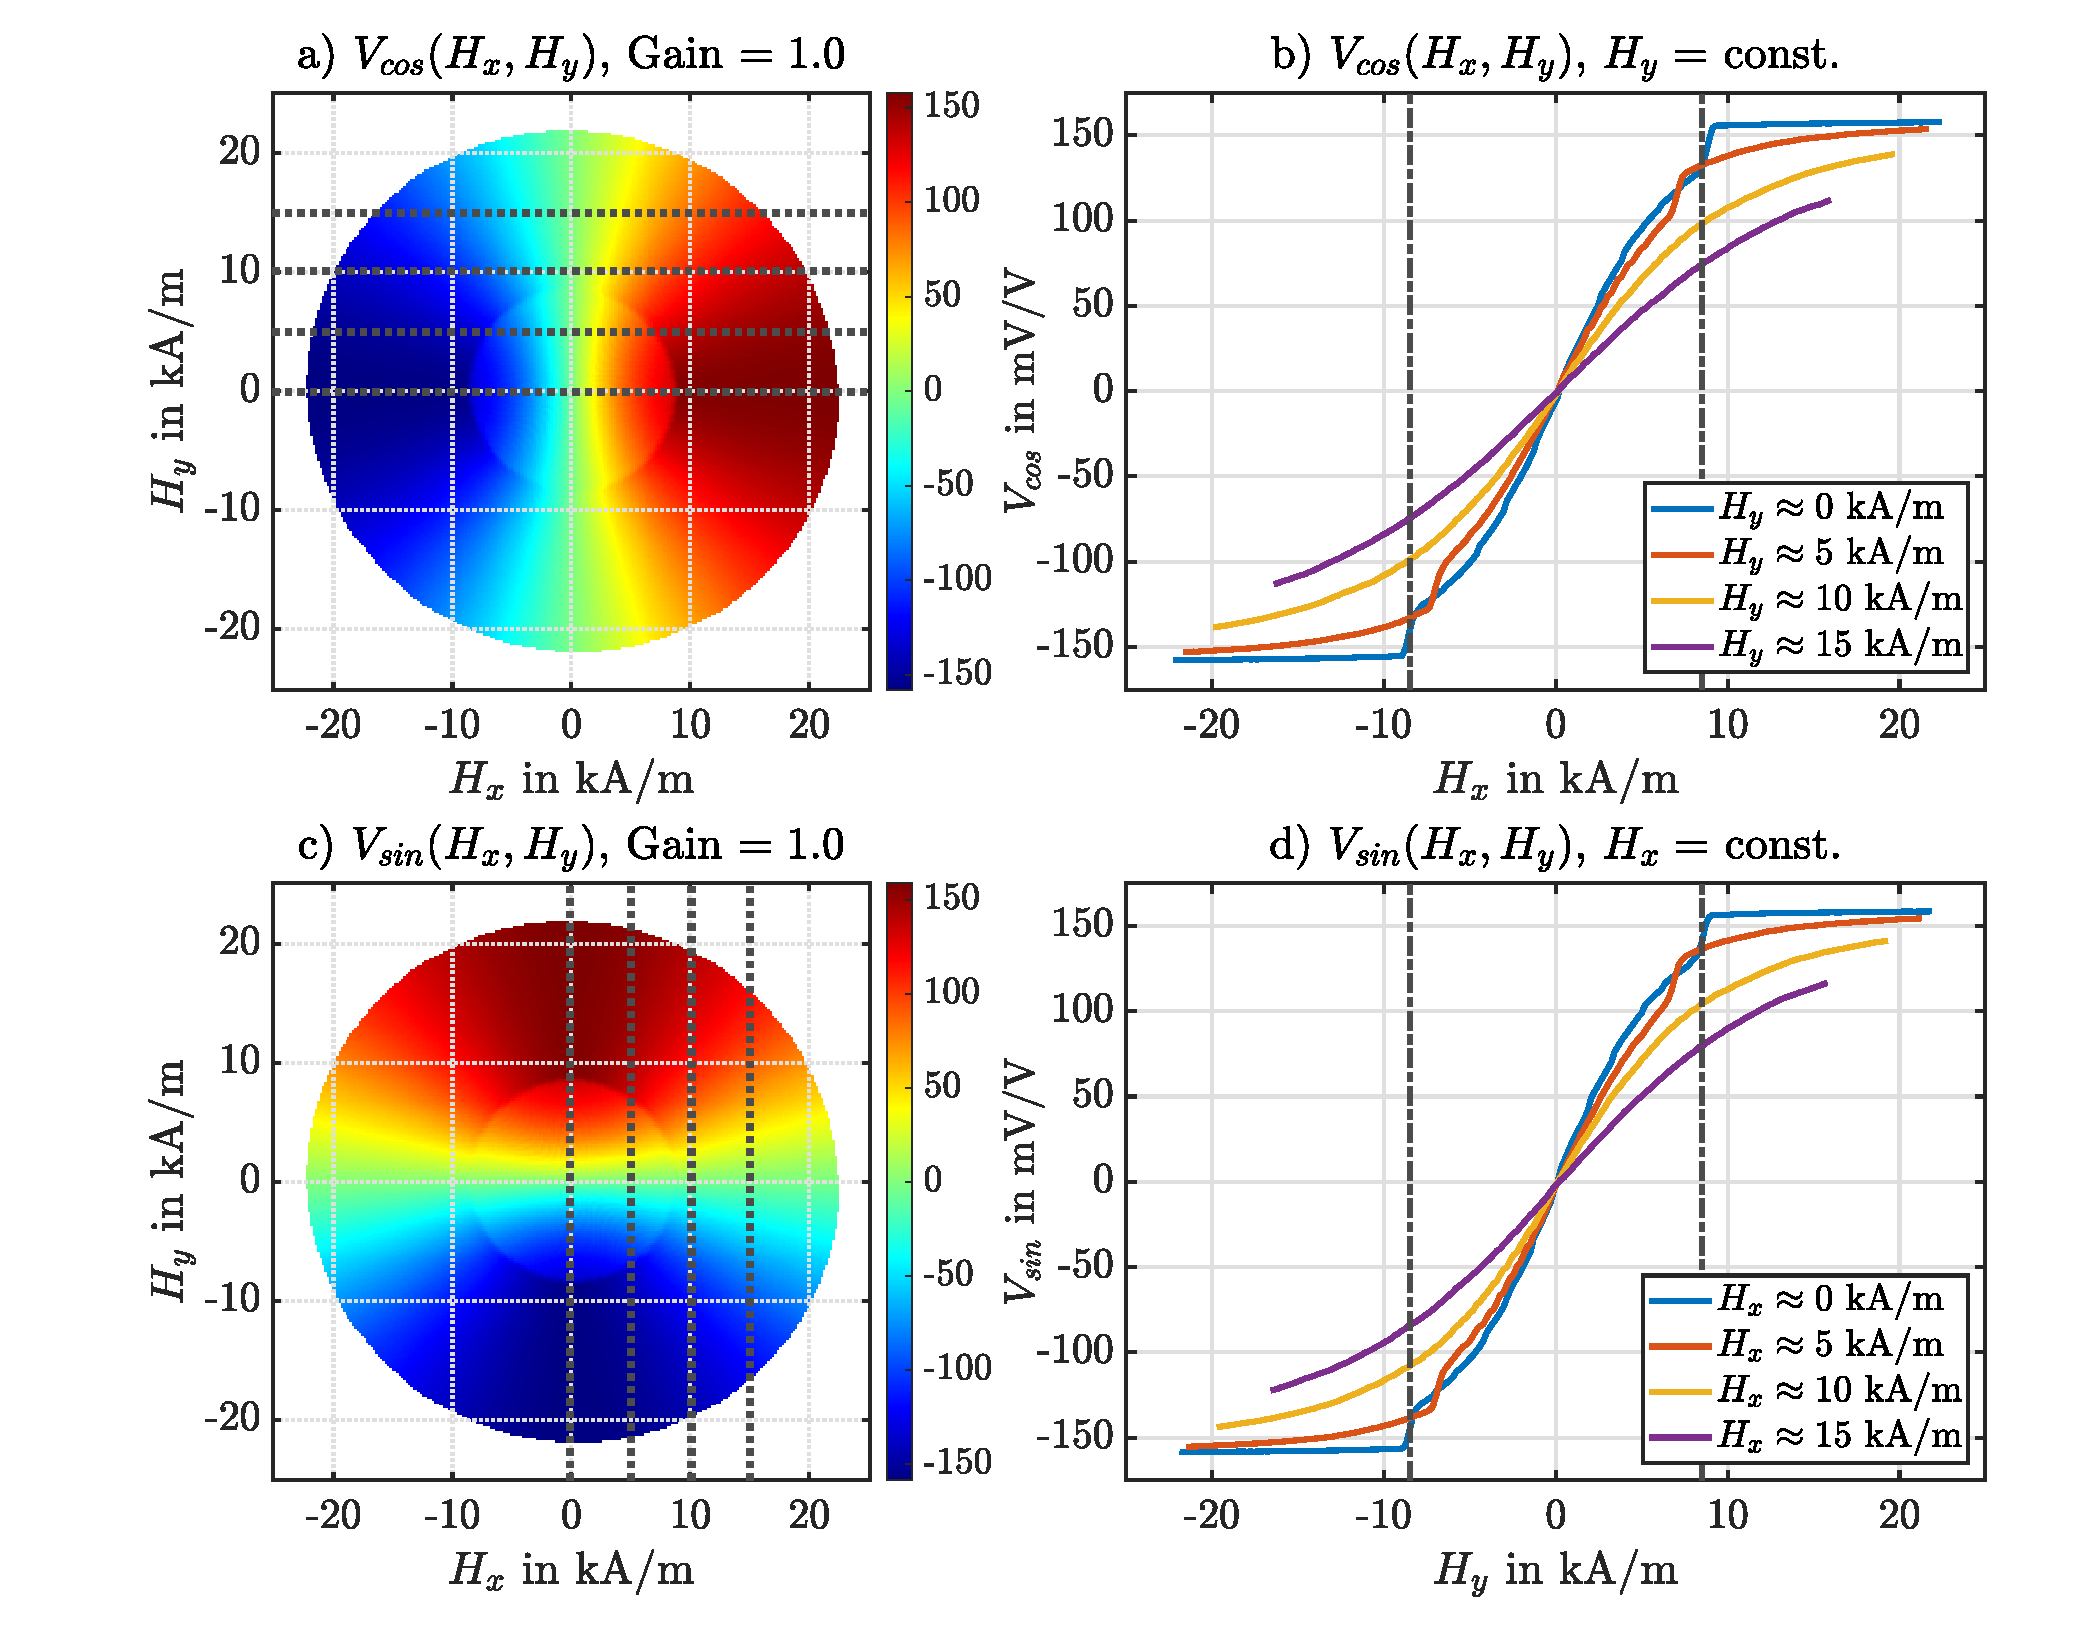
\includegraphics[width=.95\linewidth]{appendix/images/3-TDK/TDK_Kennfeld_Steigend}
	\caption[TDK TAS2141-AAAB Kennfeldquerschnitte]{TDK TAS2141-AAAB Kennfeldquerschnitte. Cosinus-Brücken-Kennfeld in 
	a) und Sinus-Brücke in c). In b) und d) sind folgend der Verdrehung Querschnitte aus a) und c) aufgetragen. In b) 
	$V_{cos}$ f. variable $H_x$- und verschieden konst. $H_y$-Feldstärken. In d) vice versa für $V_{sin}$ mit 
	verschieden konst. $H_x$- bei variablen $H_y$-Feldstärken. Breite lineare Plateaus liefern einen annähernd linearer 
	Arbeitsbereich in c) und d) zw. $\pm\SI{8,5}{\kilo\ampere\per\metre}$ f. Übertragungskennlinien $H_{x,y} = 
	\SI{0}{\kilo\ampere\per\metre}$. Grafik aus \cite{Schuethe2019}.}
	\label{fig:tdkkennfeldsteigend}
\end{figure}

%% !TEX root = ../thesis.tex
% appendix NXP KMZ60 char dataset
% @author Tobias Wulf
%

\chapter{NXP KMZ60 Kennfelddatensatz 0.0.1 29.03.2021}\label{ch:kmz60-datensatz}


\begin{figure}[tbph]
	\centering
	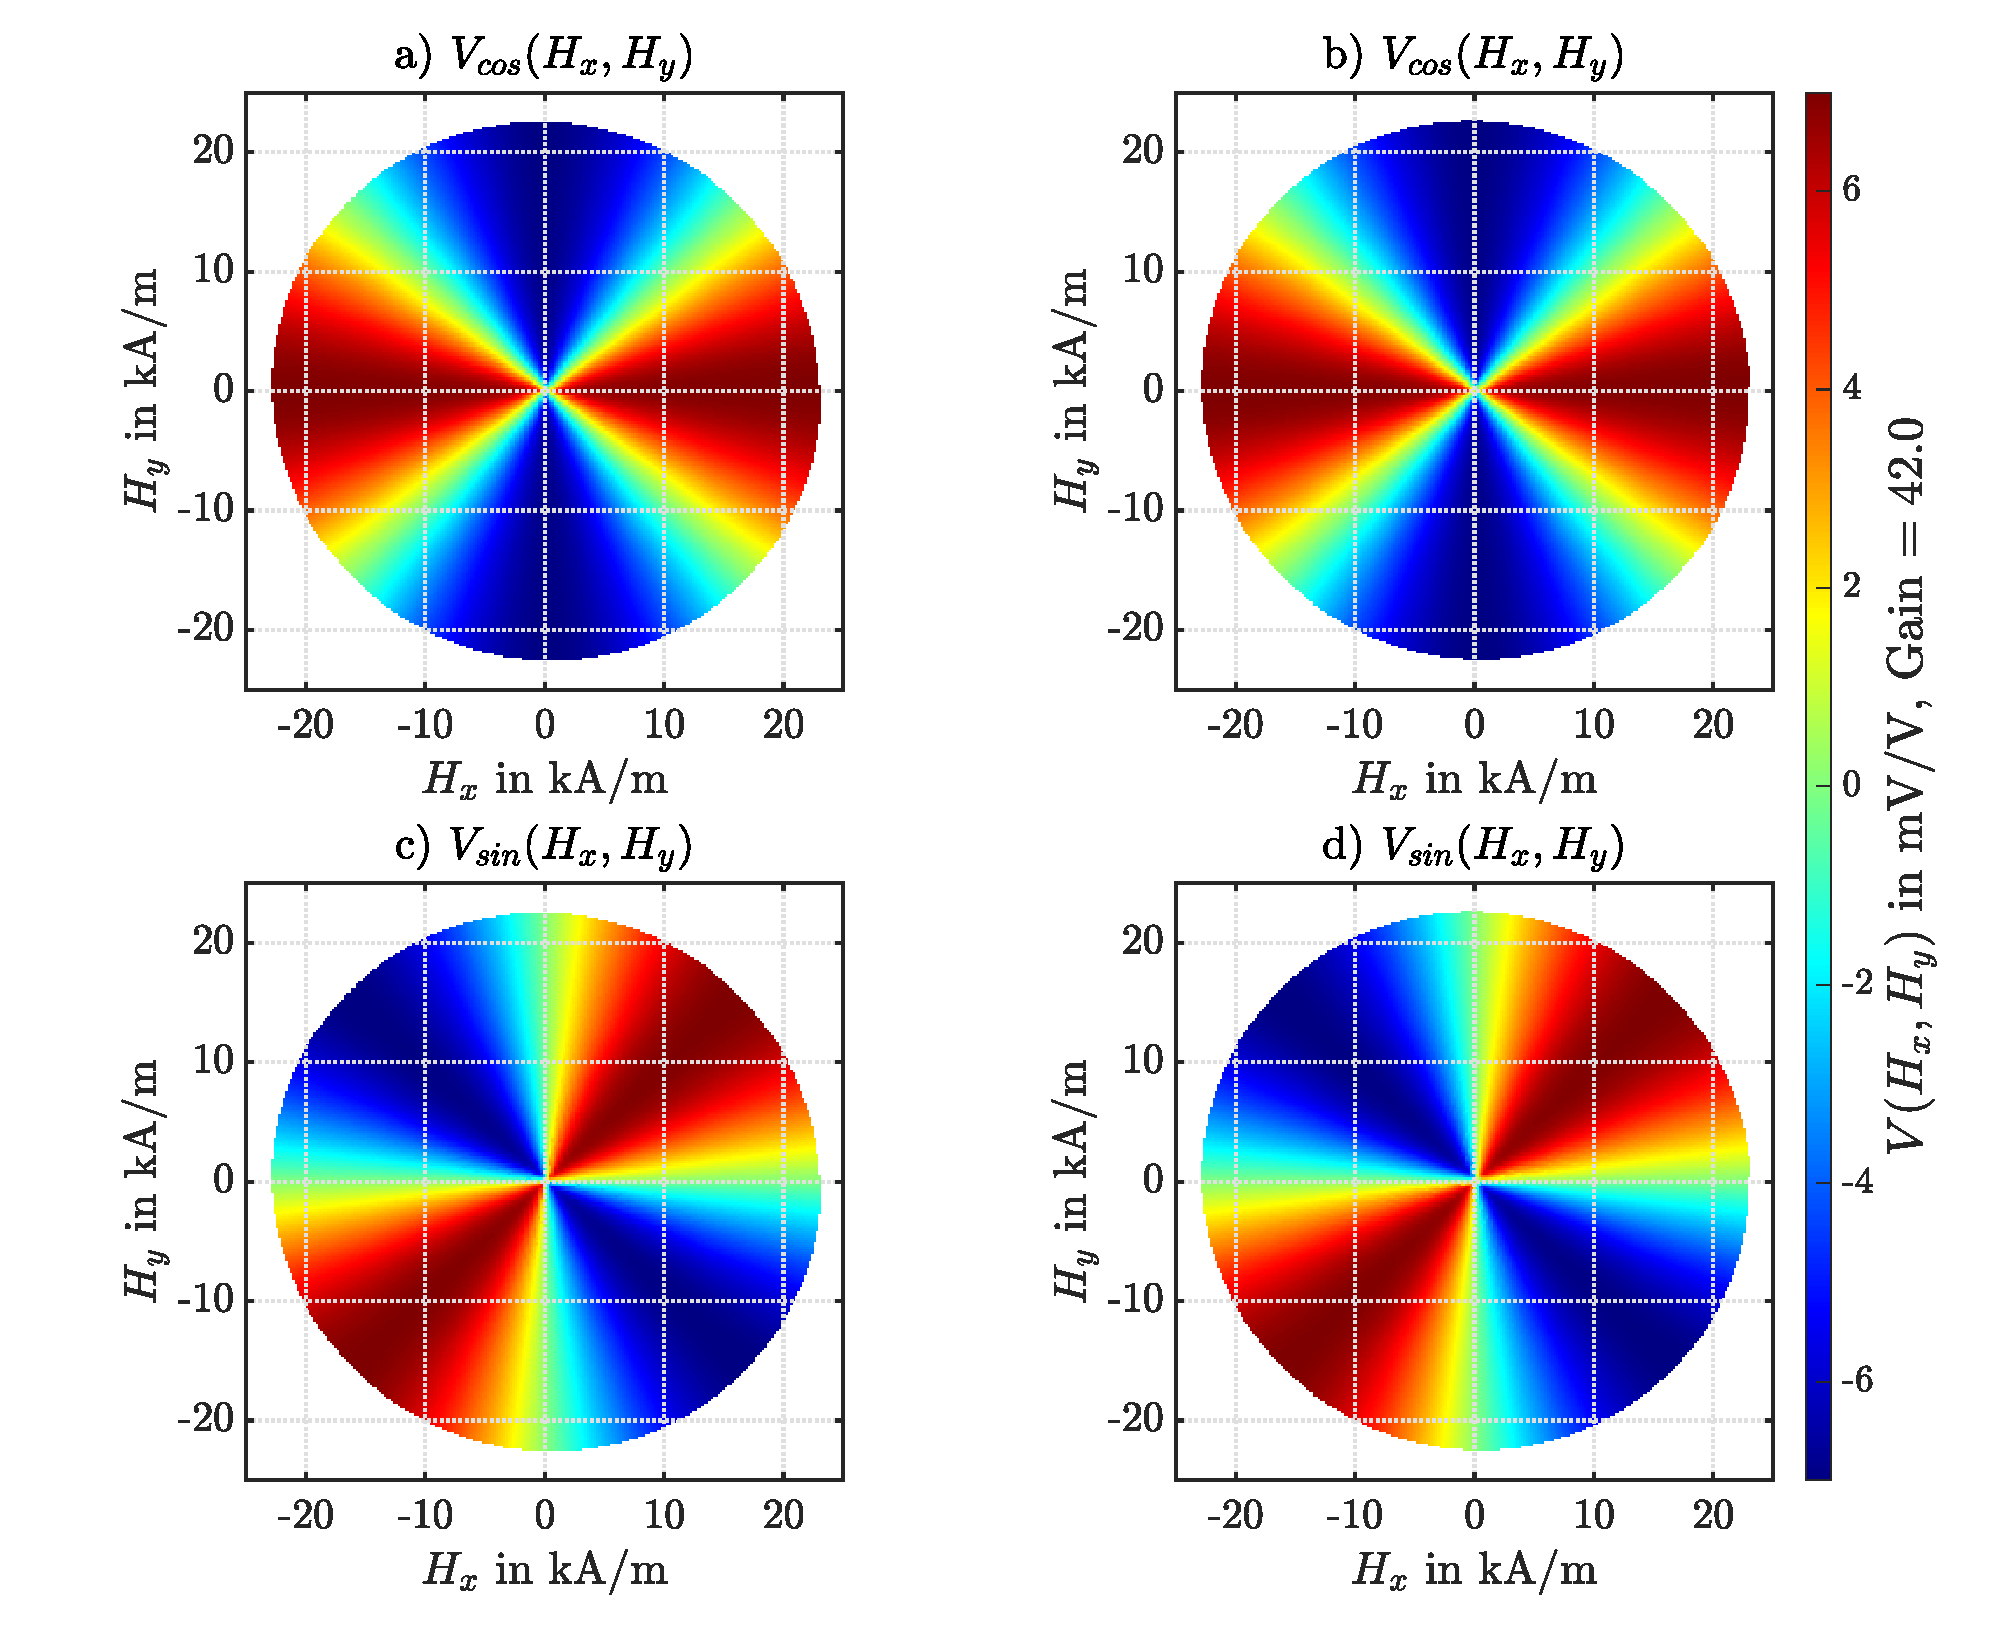
\includegraphics[width=\linewidth]{appendix/images/4-KMZ60/KMZ60_Kennfelder}
	\caption[NXP KMZ60 Winkelsensorbrückenkennfelder]{NXP KMZ60 Winkelsensorbrückenkennfelder. Zu sehen sind die 
		Kennfelder der Cosinus-Brücke a) und b). Darunter befinden sich die Kennfelder der Sinus-Brücke c) und d). 
		Die Kennfelder für beide Brücken a) und c) beziehen sich auf die steigenden Flanke der Amplitudenmodulation aus 
		\autoref{fig:magnetfeldstimuluskennfeldmethode} und die in b) bzw. d) gezeigten Kennfelder sind gewonnen aus 
		der fallenden Flanke. Die Brückenkennfelder sind normiert in $\SI{}{\milli\volt\per\volt}$. Für eine 
		Spannungsausgabe in Betriebsspannungsniveau ist eine zusätzliche Verstärkung um Faktor $42$ notwendig. Die 
		Kennfelder besitzen, jeweils in $H_x$- und $H_y$-Richtung, eine Schrittweite von 
		$\SI{0.1961}{\kilo\ampere\per\metre}$ und sind skaliert von $\SI{-25}{\kilo\ampere\per\metre}$ bis 
		$\SI{+25}{\kilo\ampere\per\metre}$. Somit ergibt sich eine Bildauflösung für ein Kennfeld von $256 \times 256$ 
		Messpunkten. Grafik nachempfunden aus \cite{Schuethe2019}.}
	\label{fig:kmz60kennfelder}
\end{figure}


\begin{figure}[tbph]
	\centering
	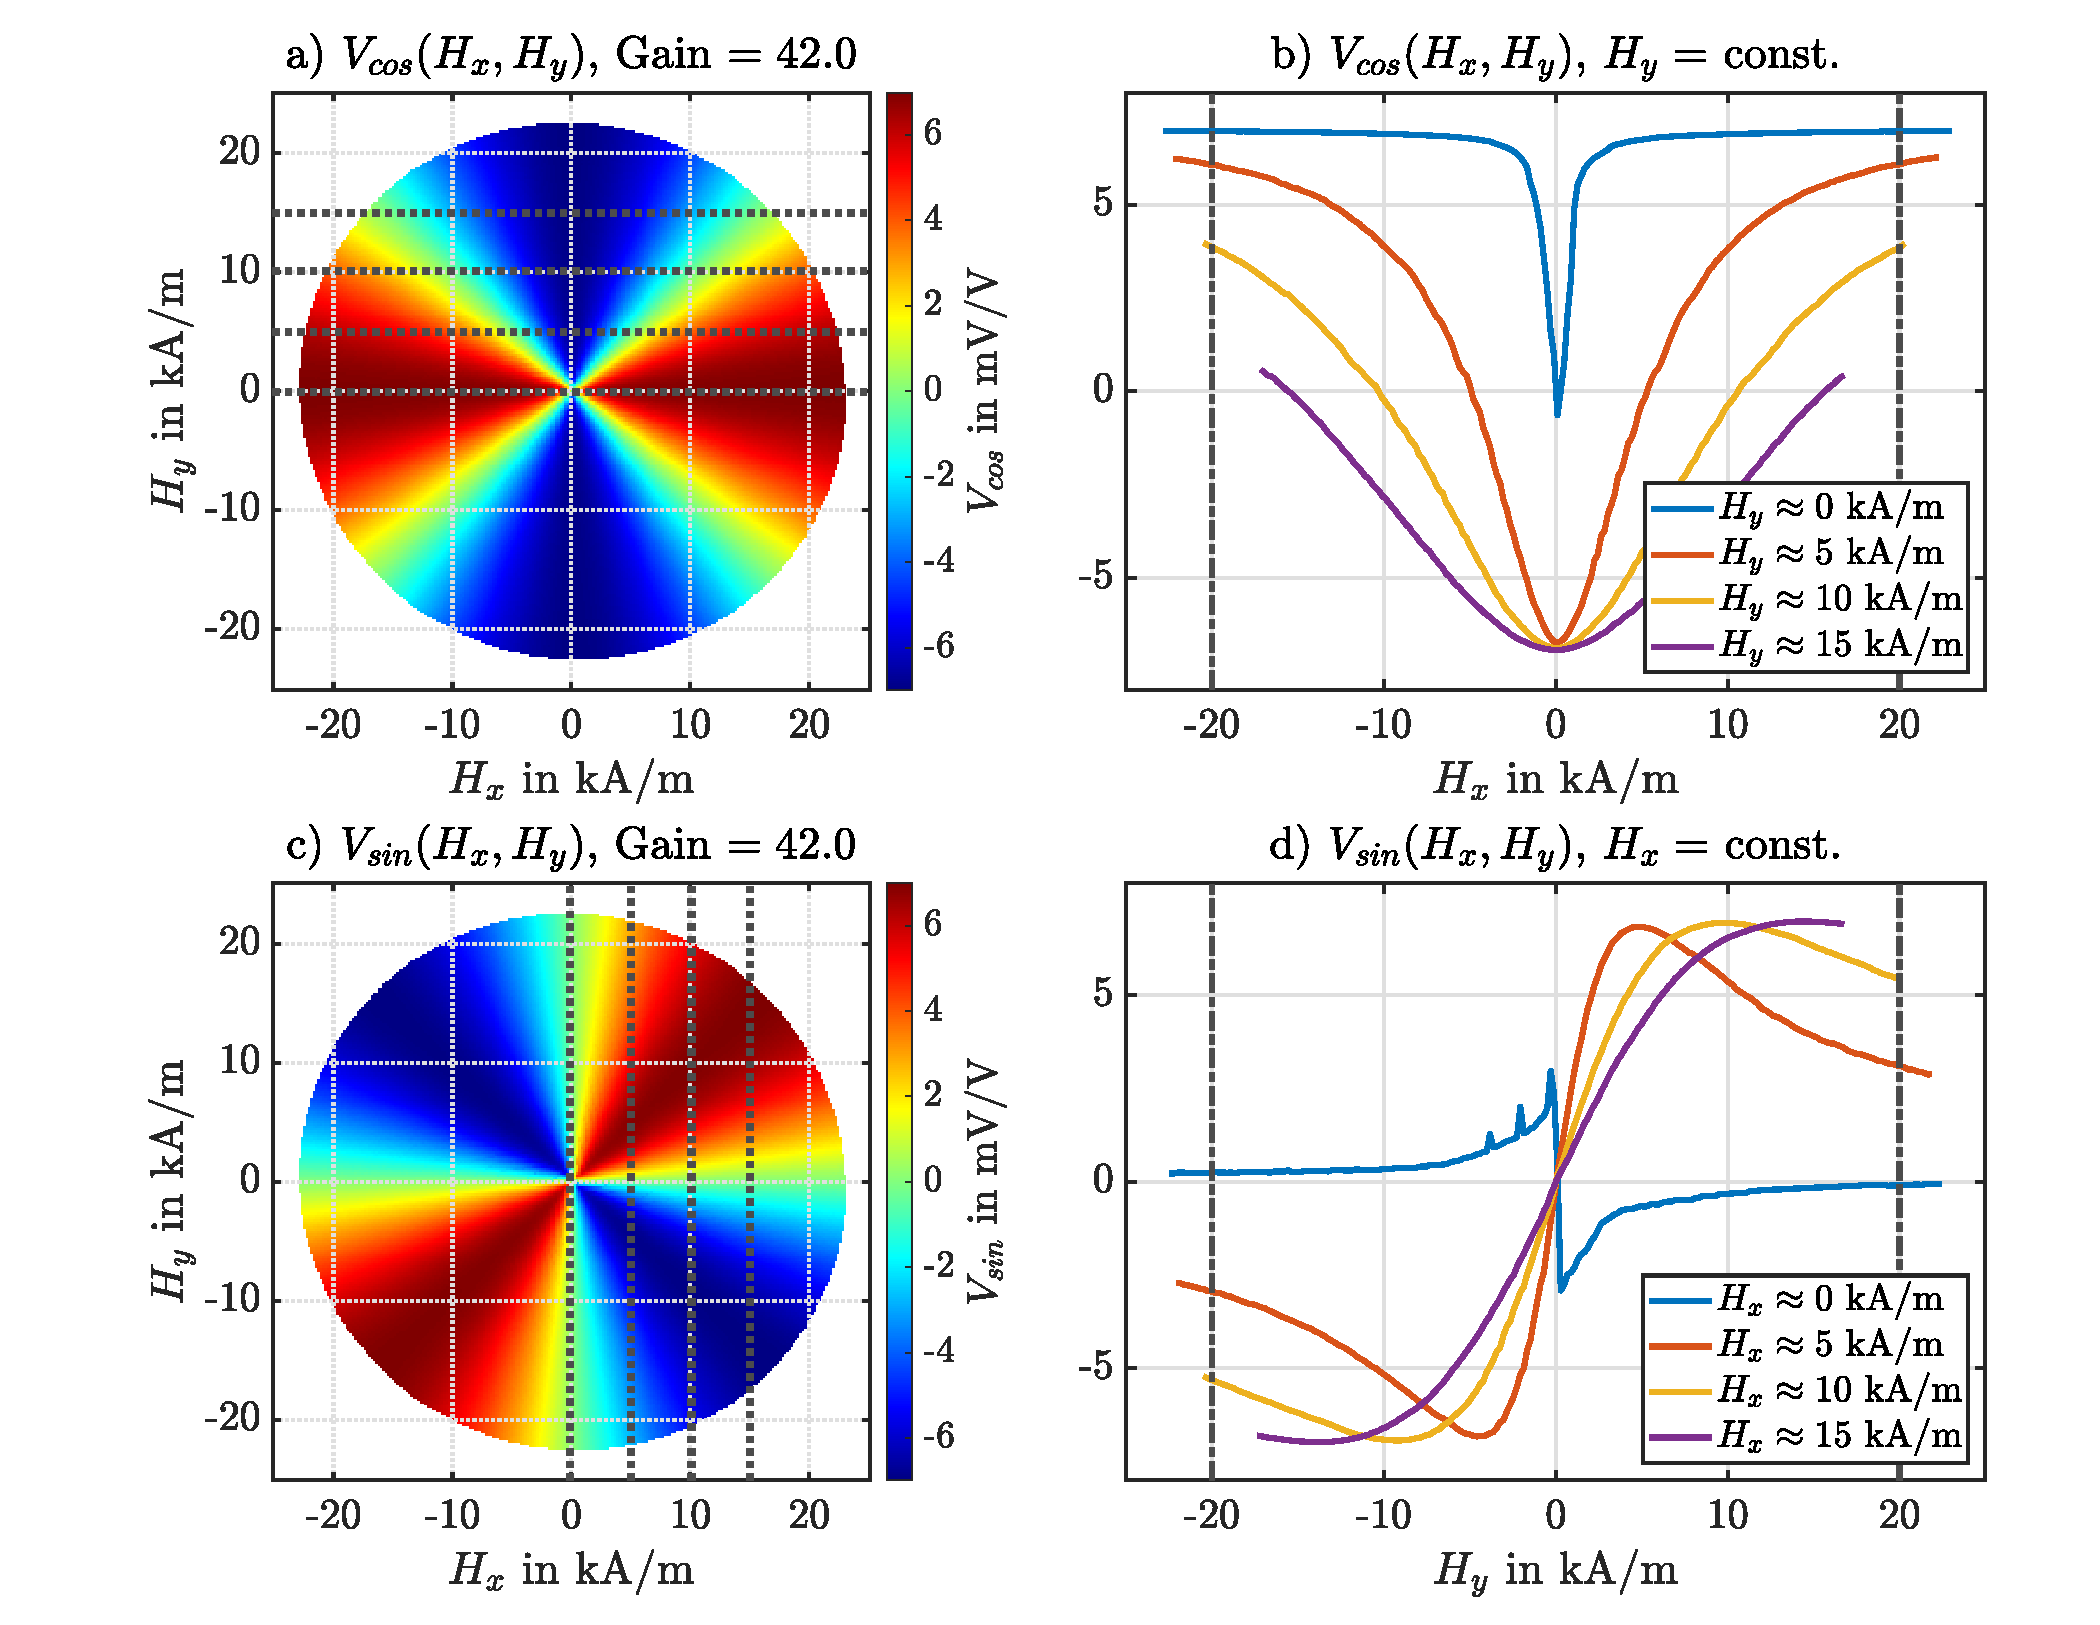
\includegraphics[width=\linewidth]{appendix/images/4-KMZ60/KMZ60_Kennfeld_Steigend}
	\caption[NXP KMZ60 Kennfeldquerschnitte]{NXP KMZ60 Kennfeldquerschnitte. Für die Kennfelder gewonnen aus 
		steigender Amplitudenmodulation a) und c). Es sind Querschnitte durch die jeweiligen Kennfelder in b) und d) 
		abgebildet. Für $V_{cos}$ a), b) verschiedene konstante $H_y$ und $V_{sin}$ c), d) entsprechend verschiedene 
		konstante $H_x$ Querschnitte. Grafik nachempfunden aus \cite{Schuethe2019}.}
	\label{fig:kmz60kennfeldsteigend}
\end{figure}




\begin{figure}[tbph]
	\centering
	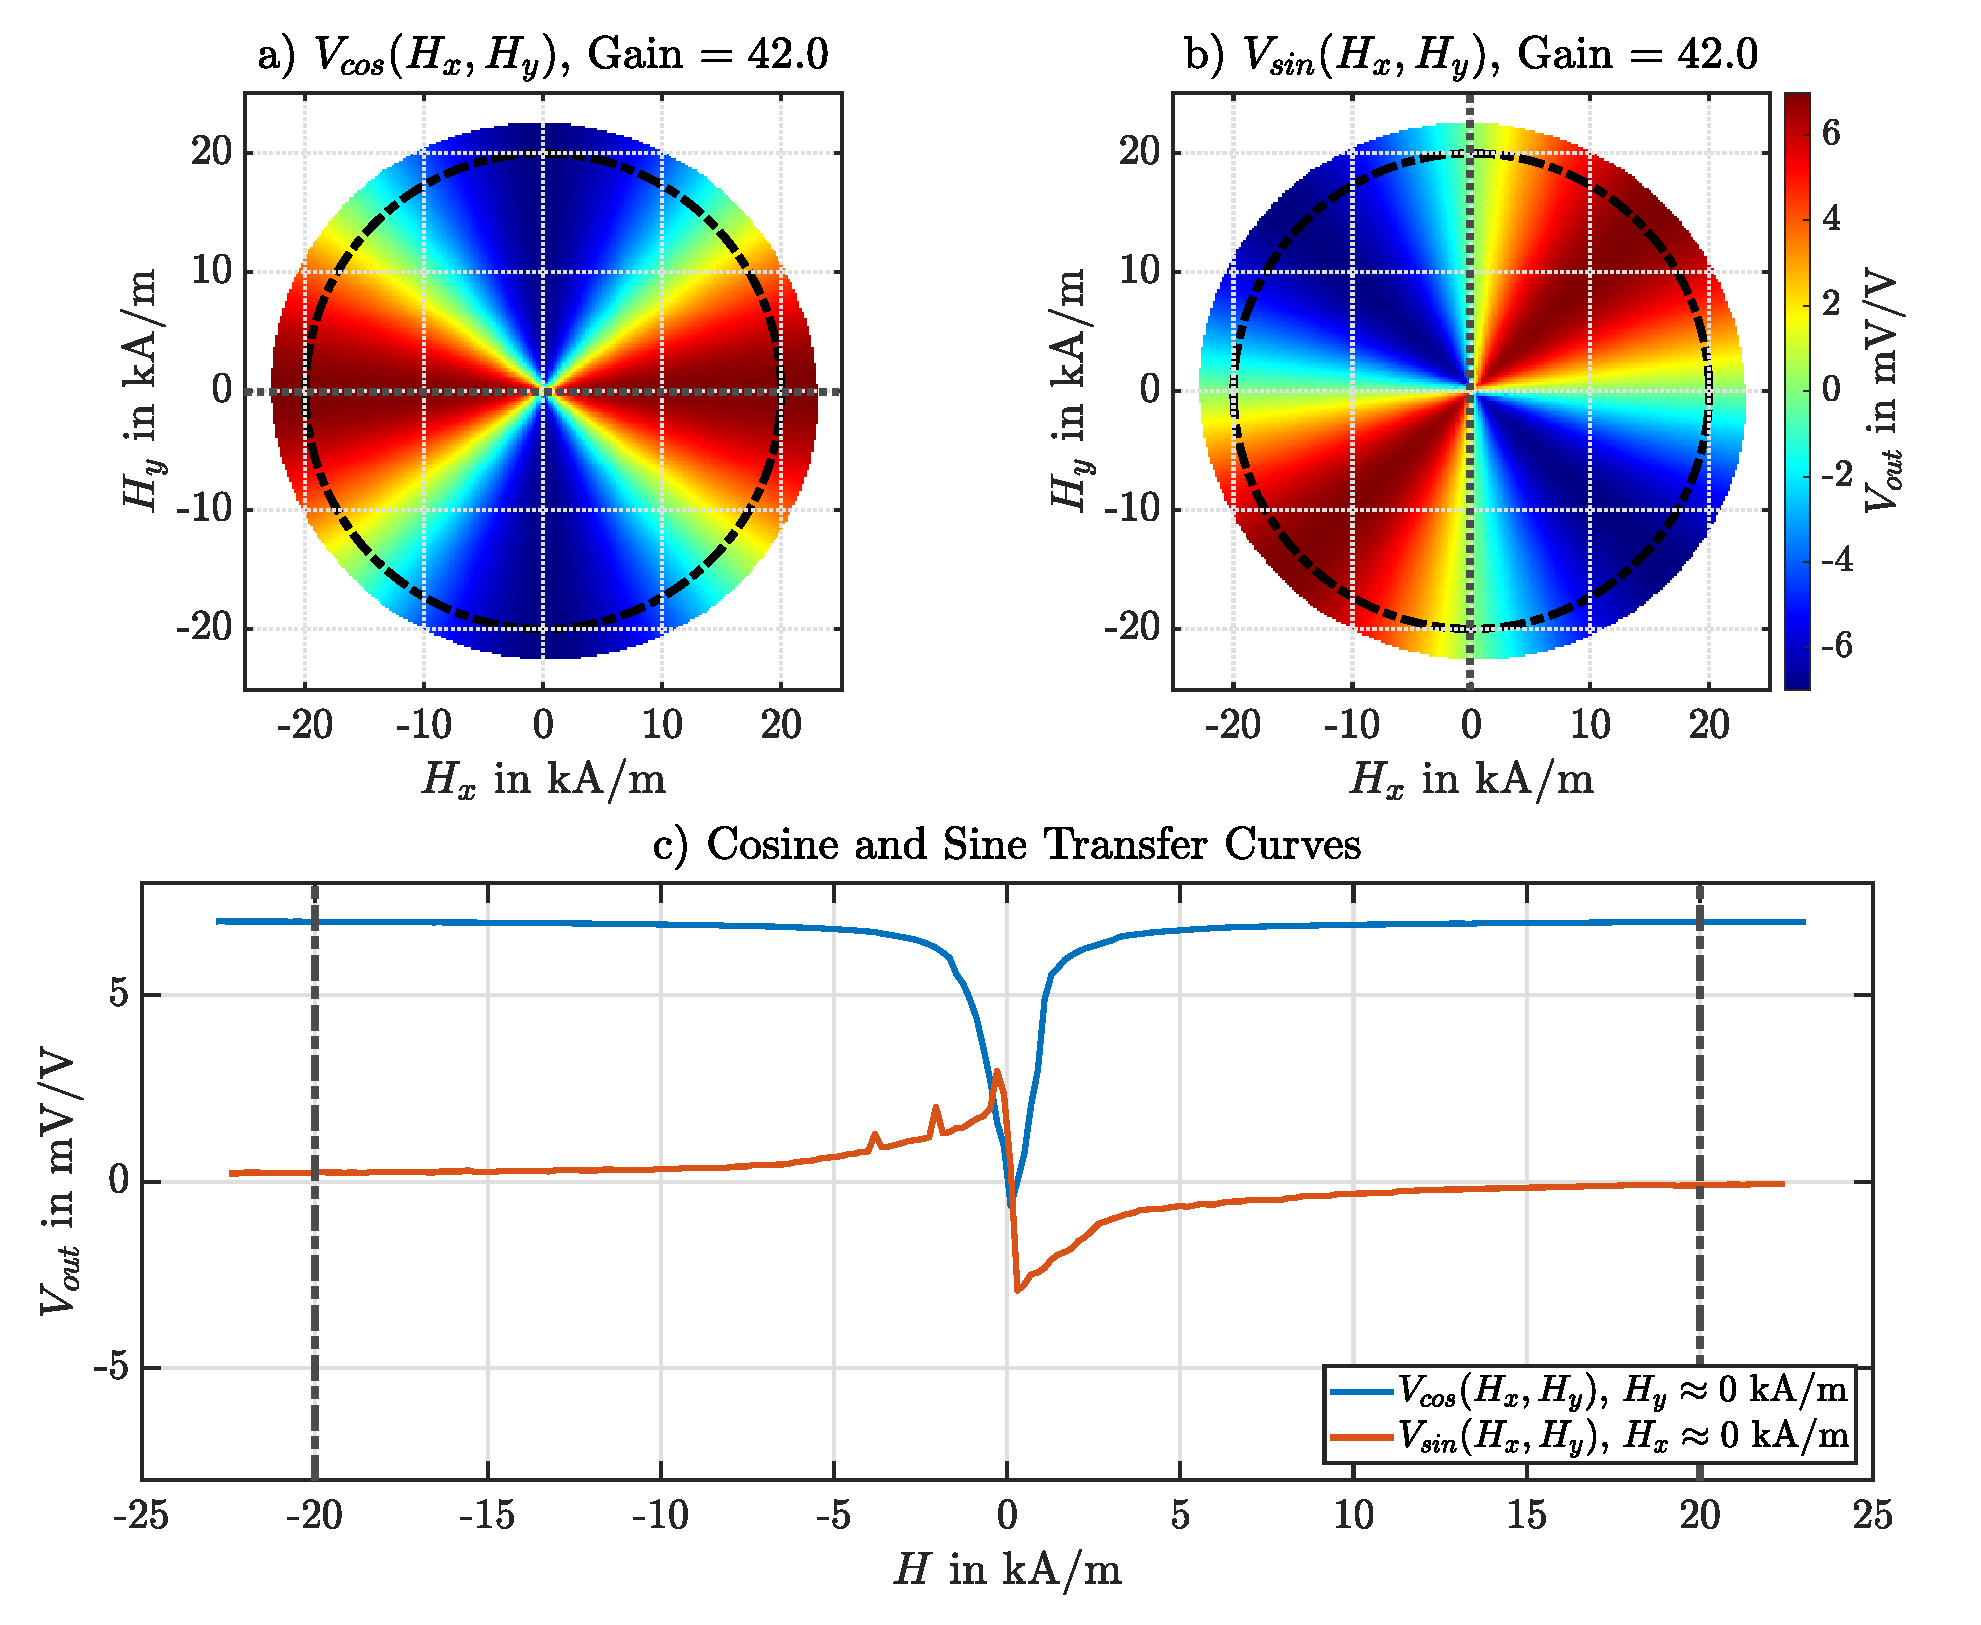
\includegraphics[width=\linewidth]{appendix/images/4-KMZ60/KMZ60_Uebertragungskennlinien}
	\caption[NXP KMZ60 Übertragungskennlinie]{NXP KMZ60 Übertragungskennlinie. Es sind wieder die Kennfelder aus 
		der steigenden Amplitudenmodulation in a) und b). In c) sind die Übertragungskennlinien für den Sensor gezeigt 
		mit Kennzeichnung für den Betrieb in Sättigung bei $\SI{20}{\kilo\ampere\per\metre}$. Ebenfalls zu sehen in a) 
		und b) durch die sich ergebene Kreisbahn mit einem Radius des aufgelegten Intervalls aus c). Grafik 
		nachempfunden aus \cite{Schuethe2019}.}
	\label{fig:kmz60uebertragungskennlinien}
\end{figure}

% !TEX root = ../thesis.tex
% appendix used software
% @author Tobias Wulf
%
\chapter{Genutzte Software 0.0.3 08.01.2021}\label{ch:genutzte-sw}

Für die Nachvollziehbarkeit der getätigten Entwicklungsarbeiten und die Erstellung der Bachelor-Thesis, ist das dafür jeweilige \gls{ac:os}
und die verwendete \gls{ac:sw} tabellarisch aufgeführt. Es finden sich genutzte Versionen der SW und Angaben zur Minimalanforderung für deren
Nutzung. Die Anforderungen sind für \gls{ac:cpu}, \gls{ac:ram}, \gls{ac:hdd} näher aufgeschlüsselt. Die Programmierarbeiten mit MATLAB sind
jeweils mit Windows und Linux geschrieben bzw. getestet worden.

\vspace{5mm}
\begin{table}[!htbp]
\centering
\resizebox{\textwidth}{!}{
\begin{tabular}{@{}lllll@{}}
\toprule
\textbf{Software}     & \textbf{Verwendungszweck (Typ)} & \textbf{Min.-Anforderung}    & \textbf{Version} & \textbf{Erscheinungstag} \\ \midrule
Ubunut Budgie         & Linux-Betriebssystem            & 2 GHz Dual-Core-CPU          & 18.04 LTS        & 26.04.2018               \\
                      & (Laptop OS)                     & 4 GB RAM                     &                  &                          \\
                      &                                 & 25 GB freier HDD-Speicher    &                  &                          \\ \hline
Windows 10 Enterprise & Windows-Betriebssystem          & 1 GHz Core-CPU               & 1909             & 12.11.2020               \\
                      & (Laptop OS)                     & 1 GB RAM                     &                  &                          \\
                      &                                 & 32 GB freier HDD-Speicher    &                  &                          \\ \hline
MATLAB                & Simulationssoftware             & Intel/ AMD x86-64 CPU        & 2020b            & 17.09.2020               \\
                      & (Multi-Paradigmen Programmier-  & 4 GB RAM                     &                  &                          \\
                      & Sprache, IDE)                   & 3.5 GB freier HDD-Speicher   &                  &                          \\ \hline
Git                   & Versionierung                   & -                            & 2.29             & 29.10.2020               \\
                      & (Kommandozeilenprogramm)        & -                            &                  &                          \\
                      &                                 & -                            &                  &                          \\ \hline
Inkscape              & Vektorgrafikzeichenprogramm     & 1 GHz CPU                    & 0.92.3           & 11.03.2018               \\
                      & (Grafikaufbereitung)            & 256 MB RAM                   &                  &                          \\
                      &                                 & 302 MB freier HDD-Speicher   &                  &                          \\ \hline
Texstudio             & Textbearbeitung f. LaTeX        & -                            & 2.12.6           & 25.07.2020               \\
                      & Dokumente (Editor)              & -                            &                  &                          \\ 
                      &                                 & 24.7 MB freier HDD Speicher  &                  &                          \\ \hline
wkhtmltopdf			  & HTML- zu Pdf-Konvertierung      & -                            & 0.12.6           & 11.06.2020               \\
                      &                                 & -                            &                  &                          \\
                      &                                 & -                            &                  &                          \\ \hline
JabRef				  &	Literaturverwaltungsprogramm    & -							   & 5.1              & 30.08.2020               \\
                      & f.BibLaTeX (Editor)             & -                            &                  &                          \\
                      &                                 & -                            &                  &                          \\
\bottomrule		
\end{tabular}}
\caption[Genutzte Software]{Genutzte Software zur Erstellung der Thesis und Dokumentation der Ergebnisse, Entwicklungsumgebung für die
geschriebene Simulationssoftware zur Generierung und Auswertung der Sensor-Array-Simulation.}
\label{tab:sw}
\end{table}

% !TEX root = ../thesis.tex
% appendix software documentation (autogenerated)
% @author Tobias Wulf
%
\chapter{Software-Dokumentation 0.0.4 13.01.2021}\label{ch:sw-doku}

Die Software-Dokumentation ist automatisiert mit MATLAB-Skripten erstellt worden.
Es ist dafür ein zweistufiger Prozess implementiert, der im ersten Schritt eine
in MATLAB integrierte HTML-Dokumentation erstellt und im Anschluss diese zu
eigenständigen PDF-Dateien exportiert. Als letzter Schritt sind diese zu einem LaTeX-Manual
zusammengefasst im Anhang eingebunden. Mit diesem Verfahren ist es möglich,
eine Dokumentation direkt aus geschriebenen M-Dateien zu generieren. Allerdings
ist es dafür nötig, eine spezielle Formatierung und einen gewissen Programmierstil einzuhalten \cite{Johnson2014}.
Die Dokumentation enthält neben dem erstellten Quellcode eine Reihe von Arbeitsanweisungen,
wie mit der Software umzugehen ist. Zusätzlich sind Beschreibungen für die Erstellung und Pflege
des Software-Projektes mit beigefügt. Die geschriebene Software ist mithilfe
des Software-Versionierungsprogramms Git erstellt worden, was eine genaue Nachvollziehbarkeit in Bezug
auf die einzelnen Arbeitsschritte ermöglicht. Zur Versionierung ist der Git-Feature-Branch-Workflow \cite{Bitbucket2020}
angewandt worden. Aus stilistischen Gründen ist die gesamte Software-Dokumentation in Englisch verfasst.

% \subimport{../../Manual/}{Manual.tex}



\Istatement

\end{document}
